\documentclass[UTF8,a4paper,12pt,fontset=fandol]{ctexart}
\usepackage{amsmath,amssymb}
\usepackage{graphicx}
\usepackage{float}
\usepackage{caption}
\usepackage{booktabs,tabularx,longtable,array}
\newcolumntype{Y}{>{\raggedright\arraybackslash}X}
\newcolumntype{P}[1]{>{\raggedright\arraybackslash}p{#1}}
\newlength{\reviewtablewidth}
\DeclareCaptionFont{reviewcaption}{\zihao{5}\songti}
\captionsetup{font=reviewcaption}
\numberwithin{equation}{section}
\usepackage[margin=2.5cm]{geometry}
\usepackage[numbers,super,sort&compress]{natbib}
\renewcommand{\bibfont}{\zihao{5}\songti}
\setlength{\bibsep}{0pt}
\usepackage[unicode,hidelinks]{hyperref}
\setcounter{secnumdepth}{3}
\ctexset{section={format=\Large\bfseries},subsection={format=\large\bfseries}}
\pagestyle{plain}

\title{\heiti\zihao{3}给定偏好下的多目标序贯决策体系研究现状及探讨}
\author{}
\date{}

\begin{document}
\maketitle

% !TeX root = main.tex
\section{引言}\label{sec:intro}

能源系统运行、生产调度和交通管理等任务需要同时考虑效率、成本与能耗等目标。节能驾驶中速度与能耗的权衡、基础设施维护中成本与失效风险的权衡，都是这类问题的具体实例\cite{he2023,remmerden2025}。这些目标之间存在冲突，一个目标的改善往往以其他目标变差为代价。这类任务还是序贯的：当前动作除了产生即时结果，还会改变系统状态，从而影响后续可采取的动作及其后果。例如，在具有储能或热惯性的能源系统中，降低当前运行功率可以减少即时能耗，却可能改变系统后续状态，增加之后恢复或补偿运行的成本。策略的优劣因此要依据一系列动作产生的长期结果来判断。多目标序贯决策要回答的，就是在系统持续演化的过程中如何选择策略，从而在多个相互冲突的目标之间取得权衡。

对于一组互不支配的候选策略，Pareto 最优性只说明它们之间不存在支配关系，并不能确定选哪一个；实际决策还需要决策者对不同目标的取舍要求，即偏好。权重、效用函数、参考点、满意水平和目标优先级等形式，可以从不同角度表达这种取舍\cite{wang2017}。本文研究偏好已经给定的情形，即决策者的取舍依据是决策问题的已知输入，讨论如何把它纳入多目标序贯决策的建模、求解与评价。

偏好给定并不意味着问题已经化为单目标问题。首先要明确的是：给定偏好定义了怎样的长期决策准则，这一准则又具有怎样的序贯结构。固定线性权重下，可以在一定条件下把多维回报标量化，再用单目标序贯决策方法求解；对于更一般的偏好，长期准则未必具有阶段可加性，当前环境状态也可能不足以支持后续决策，需要引入累计回报、扩展状态、回报分布等专门的表示与求解机制。具体求解研究已经说明了这一点：累计回报上的非线性效用推动了保留历史结果的搜索和回报分布学习\cite{hayes2023,reymond2023}，严格优先关系要求策略更新始终维持目标之间的比较次序\cite{skalse2022}。信息条件又进一步区分了求解路线：模型已知时可以直接规划，允许交互时可以补充样本，只有固定历史数据时还要处理数据对不同权衡的支持程度，从多奖励批量价值学习\cite{lizotte2012}到偏好与回报条件化的离线策略\cite{zhu2023}，数据覆盖始终是这类方法的适用边界。

已有综述从不同角度整理了这一领域。Roijers 等从三种无法、难以或不宜把多目标问题转化为单目标问题的场景出发，按场景、标量化函数的性质和所考虑的策略类型建立分类，据此确定最优解应是单个策略、凸包还是 Pareto 前沿，并按这一分类综述规划与学习方法\cite{roijers2013}。Hayes 等面向希望采用多目标视角的研究者和实践者，提出以用户效用为中心的设计流程：先收集效用信息、确定允许的策略类型，再推出解的概念并选择算法；该文讨论了 SER 与 ESR 的选择依据和策略类型的影响，并对算法和评价指标作了简要综述\cite{hayes2022}。Wang 等的近期综述从理论基础、算法框架、评价基准和应用几个方面总结多目标强化学习研究，按模型可用性、策略范围和偏好表示对算法分类，涵盖基于模型的规划、无模型学习和交互式偏好获取\cite{wang2026}。

现有综述主要围绕"需要求出什么样的解"和"有哪些算法"来组织文献。对于偏好已经给定的问题，仍有三个方面值得专门梳理。其一，给定偏好形成的长期准则不只是 SER 与 ESR 的选择，还包括评价对象、时间聚合方式、优先关系和可接受性要求，它们共同决定了求解时必须保留哪些信息。其二，模型可用、允许交互和只有固定历史数据三类信息条件下，同一准则的求解方法和理论保证差别很大；上述综述的算法分类没有把固定历史数据单列为一类条件。其三，策略库和条件策略等多策略方法在给定偏好问题中的作用是复用计算和数据，对它们的评价最终要落实到每个给定偏好下实际选出的策略。

围绕这三个方面，本文做了以下工作：
\begin{enumerate}
\item 提出“长期准则---信息表示---策略类别---模型与数据条件”四维分析框架，把偏好表达、评价对象、时间聚合和随机性处理统一为长期决策准则，并据此分析各类准则的可分解性、状态充分性、递推结构和所需策略类别。
\item 按模型可用、允许交互和固定历史数据三类信息条件组织求解方法，每类条件下再按准则类型比较方法的机制与保证范围，并将跨偏好方法单独作为复用机制讨论。
\item 从原准则出发讨论单策略、策略集合与条件策略的评价，以及离线评价、实验规范和应用证据的层次，并据此提出四个研究方向。
\end{enumerate}

全文共八章。第~\ref{sec:framework}~章先界定研究范围并给出分析框架；第~\ref{sec:criteria}~章讨论给定偏好如何形成长期决策准则，第~\ref{sec:structure}~章在此基础上分析准则的序贯结构与求解条件。随后，第~\ref{sec:solving}~章按三类信息条件比较求解路线，第~\ref{sec:evaluation}~章回到准则本身，讨论策略评价与应用证据。第~\ref{sec:future}~章提出未来研究方向，最后一章总结全文。

% !TeX root = main.tex
\section{研究范围与分析框架}\label{sec:framework}

\subsection{研究范围}\label{sec:framework-scope}

本文讨论偏好已作为输入给定的多目标序贯决策问题。这里的给定偏好可以是固定权重、非线性效用、目标优先关系或可接受性要求；而环境模型是否已知，则是与偏好无关的另一项信息条件。本文不讨论如何从比较反馈或示范中识别未知偏好，也不把一般静态多目标优化方法当作序贯问题的求解方法；静态标量化函数和解集指标只在用于构造长期准则或评价策略时讨论。

\subsection{基本模型}\label{sec:framework-model}

多目标 Markov 决策过程（MOMDP）是基本的建模形式。系统处于状态 $S_t$ 时选择动作 $A_t$，随后产生下一状态 $S_{t+1}$ 和多维回报 $\mathbf R_t\in\mathbb R^m$，其中 $m$ 为目标数。在完全观测且具有 Markov 性的情形下，下一状态和回报的条件分布由当前状态与动作决定；给定初始状态分布 $\rho_0$、评价时域及时间聚合规则后，策略决定了长期结果的分布\cite{roijers2013}。这一框架不要求模型能被求解器直接调用；状态只能部分观测时，策略要依据可用观测或信念状态做决策。

设 $h_t$ 为截至时刻 $t$ 决策者可获得的信息，策略一般写为 $\pi_t(a\mid h_t)$。相对于环境状态的 Markov 策略只依赖当前状态，历史依赖策略还可以利用累计回报、剩余预算等信息；是否允许动作随机化、时间依赖和记忆，都属于策略集合 $\Pi$ 的定义。对于有限时域折扣累计回报，记
\begin{equation}
\mathbf G^\pi=\sum_{t=0}^{T-1}\gamma^t\mathbf R_t,
\end{equation}
下文用小写 $\mathbf r_t$ 表示 $\mathbf R_t$ 的实现值。给定偏好 $p$ 后，需要规定如何评价这一随机向量或其他轨迹结果，再在允许的策略集合内比较策略。期望回报向量、完整结果分布和路径事件保留的信息各不相同，在评价准则确定之前不能相互替代\cite{hayes2022}。

图~\ref{fig:problem-overview}~展示了策略执行如何产生多维结果，以及给定偏好如何参与长期准则的定义。

\begin{figure}[H]
\centering
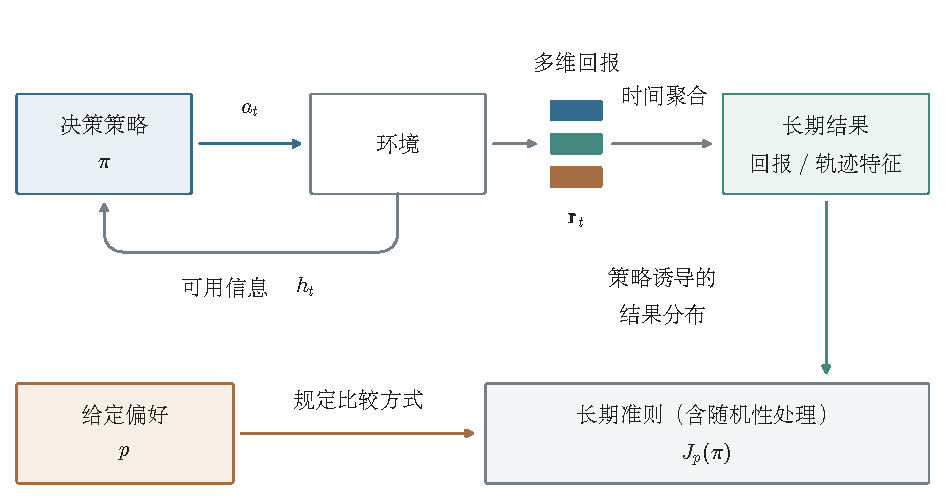
\includegraphics{figures/problem_overview.pdf}
\caption{给定偏好下的多目标序贯决策问题。策略依据可用信息 $h_t$ 选择动作 $a_t$，环境产生多维回报 $\mathbf r_t$，时间聚合形成长期结果。给定偏好、时间聚合与随机性处理共同规定策略比较准则 $J_p(\pi)$；图中的回路描述策略执行，不限定训练时的模型与数据来源\cite{hayes2022}。}
\label{fig:problem-overview}
\end{figure}

\subsection{分析框架}\label{sec:framework-dimensions}

围绕上述模型，本文从四个维度分析给定偏好下的多目标序贯决策问题。

\begin{enumerate}
\item \textbf{长期准则}：偏好以什么形式表达，作用于阶段结果、累计结果还是轨迹特征，跨阶段如何聚合，随机结果如何评价。这四项共同决定策略之间如何比较、哪些策略可以接受，由第~\ref{sec:criteria}~章展开。
\item \textbf{信息表示}：为了按长期准则比较策略，决策时必须保留哪些历史信息，价值函数要概括未来结果的哪些信息，以及这些表示是否支持递推求解。这部分在第~\ref{sec:structure-decomp}~至~\ref{sec:structure-recursion}~节讨论。
\item \textbf{策略类别}：最优解是否需要随机化、记忆或时间依赖，实际部署允许哪一类策略。策略类别问题在第~\ref{sec:structure-policy}~节处理。
\item \textbf{模型与数据条件}：环境模型是否可用、能否新增交互、历史数据记录了什么并覆盖了哪些区域。它决定前三个维度所需的信息从哪里获得，第~\ref{sec:solving}~章按这一维度组织求解方法。
\end{enumerate}

这四个维度并非并列，而是有先后关系：长期准则决定需要保留哪些信息；信息表示和策略类别限定了可搜索的决策规则；模型与数据条件则决定这些信息能否获得、以什么代价获得。第~\ref{sec:evaluation}~章的策略评价则回到第一个维度，检验求得的策略是否实现了原准则，评价所需的信息同样受第四个维度的限制。


这一框架也给出了比较不同方法的前提。两种方法只有在长期准则（包括初始状态分布和偏好语义）、策略类别和可用信息都一致时，性能差别才能归因于求解方法本身；任何一项不同，差别都可能来自问题设定。跨偏好的策略库和条件策略在本框架中被视为复用计算与数据的手段，其质量最终要落实到每个给定偏好下实际选出的策略上（第~\ref{sec:solving-reuse}~节和第~\ref{sec:eval-sets}~节）。

% !TeX root = main.tex
\section{从给定偏好到长期决策准则}\label{sec:criteria}

给定偏好的多目标序贯决策，第一步是把决策者对目标结果的取舍要求转化为明确的策略比较准则。这一转化取决于四件事：偏好以什么形式表达，作用于什么评价对象，跨阶段的结果如何累积，以及环境的随机性如何处理。只给出偏好参数，还不足以完整刻画决策要求。

本章先讨论权重、效用、参考点、优先级和约束等偏好表达方式，再分析它们如何与时间累积和随机性结合，形成具体的长期决策准则。本文所说的“决策准则”不限于实值目标函数，也包括判定策略优劣的比较规则和界定策略可接受性的条件。

\subsection{基于实值函数的多目标结果评价}\label{sec:criteria-value}

设待评价的多维结果为
\begin{equation}
\mathbf{x}=\left(x_{1},\ldots,x_{m}\right),
\end{equation}
其中 $\mathbf{x}$ 可以是即时回报、累计回报或其他明确界定的评价对象。给定偏好参数 $p$ 后，可以用标量化函数或效用函数 $u_{p}(\mathbf{x})$ 对多维结果做实值评价，从而建立结果之间的排序\cite{wang2017,hayes2022}。本节只讨论偏好在多维结果空间中的表达方式；评价对象随机时，效用如何与期望、结果分布或风险度量组合，在第~\ref{sec:criteria-stochastic}~节讨论。

线性加权是最直接的多目标评价形式：
\begin{equation}
u_{\mathbf{w}}(\mathbf{x})
=
\sum_{i=1}^{m}w_{i}x_{i},
\qquad
w_{i}\geq 0,
\qquad
\sum_{i=1}^{m}w_{i}=1.
\end{equation}
在各目标的优化方向和尺度统一后，线性加权以固定的边际替代关系描述目标之间的补偿：对任意两个目标 $x_i$ 和 $x_j$，在 $w_j>0$ 时，相对取舍由权重之比 $w_i/w_j$ 决定。Marler 和 Arora 系统分析了权重、目标取值与最终折中解之间的关系，指出权重的实际偏好含义与目标的尺度和取值范围密切相关\cite{marler2010}。因此，脱离计量单位和尺度，权重并不能解释为各目标的“重要程度”。例如，保持权重不变而改变某个成本指标的计量单位，就可能改变结果之间的相对评价。归一化可以减弱尺度差异，但所用的归一化区间、参考值和基准同样会改变给定权重对应的实际取舍。用线性权重表达偏好时，应同时写明各目标的优化方向、计量尺度和归一化方式\cite{hayes2022}。

非线性效用函数可以描述随结果水平变化的取舍关系，以及目标之间的交互作用。对于可微效用 $u(\mathbf{x})$，目标之间的局部替代关系由边际效用之比决定，因而随 $\mathbf{x}$ 的位置变化。效用的具体形式决定了允许哪些补偿、补偿如何随结果水平改变。若希望评价与各目标预先规定的改善方向一致，可以对效用施加相应的单调性条件。

公平性准则是随结果水平改变取舍的一类具体效用。对经过尺度处理、可以共同比较的正结果，广义均值为
\begin{equation}
M_q(\mathbf x)=
\begin{cases}
\left(m^{-1}\sum_{i=1}^m x_i^q\right)^{1/q},&q\neq0,\\
\left(\prod_{i=1}^m x_i\right)^{1/m},&q=0.
\end{cases}
\end{equation}
$q=1$ 对应算术平均，$q=0$ 对应几何平均，$q\to-\infty$ 时趋于最差目标 $\min_i x_i$；这里用 $q$ 表示文献中的 $p$-mean 参数，以区别于本文通用的偏好记号 $p$。这一参数族把平均收益和对最差目标的关注放进同一组给定准则中，正值域和目标尺度是其定义条件\cite{kim2025portfolio}。广义 Gini 福利则先把结果从小到大排序，再用递减的正权重评价各排序位置，使较差的结果得到更大权重\cite{siddique2020fair}。它与为各目标固定权重的线性加权不同：某个目标得到多少边际关注，取决于它当前的排序。这些效用可以作用于单次结果，也可以作用于期望结果，采用哪种随机评价需要另外规定。

当决策者更容易给出希望达到的目标水平时，可以用参考点表达偏好。Wierzbicki 将愿望水平与成就标量化函数结合，以结果相对于参考目标的实现程度组织方案比较\cite{wierzbicki1982}。设参考点为
\begin{equation}
\mathbf{z}=\left(z_{1},\ldots,z_{m}\right),
\end{equation}
表示决策者期望达到的目标水平。参考点要与偏离度量结合才构成完整的评价规则，例如加权短缺形式
\begin{equation}
d_{\mathbf{w}}(\mathbf{x},\mathbf{z})
=
\sum_{i=1}^{m}
w_{i}\max\left(z_{i}-x_{i},0\right).
\end{equation}
它只惩罚未达到参考水平的部分，衡量实际结果相对于期望水平的短缺。若决策者还关心超额完成、最大短缺或目标之间的优先关系，可以相应调整偏差函数及其聚合方式。参考点提供评价的基准，结果之间的排序由参考点与偏差度量共同决定\cite{wang2017}。

另一种聚合方式是最小化最大加权偏差。对均需最大化的结果，令 $a_i(\mathbf x)=w_i(z_i-x_i)$，Tchebycheff 标量化及其平滑形式为
\begin{equation}
d_{\mathrm T}(\mathbf x)=\max_{1\leq i\leq m}a_i(\mathbf x),
\qquad
d_{\mu}(\mathbf x)=\mu\log\!\left(\sum_{i=1}^{m}\exp\!\left(\frac{a_i(\mathbf x)}{\mu}\right)\right),
\quad \mu>0.
\end{equation}
这里的偏差保留正负号，与只惩罚短缺的加权短缺函数语义不同。最大值聚合突出偏差最大的目标，平滑形式用可微近似代替最大值运算。Lin 等给出的界
\begin{equation}
d_{\mu}(\mathbf x)-\mu\log m\leq d_{\mathrm T}(\mathbf x)\leq d_{\mu}(\mathbf x)
\end{equation}
表明平滑参数控制了标量化值的近似误差\cite{lin2024smooth}。这个界不保证任意两个结果的排序不变：评价差距较小时，平滑可能改变比较结果。因此，把静态标量化用于长期结果评价时，应写明原偏差函数和近似参数；序贯递推条件在第~\ref{sec:structure}~章另行分析。

权重、效用函数和参考点并不是彼此独立的偏好类别，而是构造评价规则的不同要素：参考点可以是效用函数或距离函数中的参数，权重可以表示目标之间或偏差之间的相对取舍。比较这些形式时，关键在于它们如何定义评价基准、允许哪些目标补偿，以及由此形成怎样的结果排序。

\subsection{优先关系与可接受性要求}\label{sec:criteria-priority}

除了用实值函数做整体评价，决策者还可以直接规定目标之间的优先关系，或用满意水平和约束界定可接受结果的范围。这类表达限定了目标之间如何补偿、哪些结果可以接受，并可与上一节的实值评价组合使用。

词典序偏好为各目标规定严格的优先顺序：比较两个结果时先看最高优先级目标，只有它无法区分两个结果时，才比较下一优先级目标。在严格词典序下，低优先级目标的改善无法补偿高优先级目标的损失。有限权重的加权能否与词典序给出一致的排序，取决于可行结果集合、目标取值范围以及高优先级目标可能出现的最小差异。如果允许高优先级目标在一定范围内退让，可以引入容差，例如限定其相对最优水平的最大允许损失，再在满足该条件的结果中优化低优先级目标\cite{skalse2022}。

严格优先关系还涉及随机结果排序的公理基础。Shakerinava 等分析了不要求连续性公理的词典序期望效用表示\cite{shakerinava2025lex}。例如，若任何有正概率严重失效的方案都劣于任意安全方案，那么再低的失效概率也无法由其他收益补偿。这种偏好违反标量期望效用表示所需的连续性，有限的惩罚权重未必能表达它。具体的安全约束是否具有这种语义，由任务定义决定。

满意水平为一个或多个目标设定希望达到或最低可接受的水平，同一个满意水平可以有两种用法。一种把未达标的程度作为软性偏差，与其他目标上的收益一起评价；另一种把满意水平作为可接受性条件，只在达标的结果或策略中继续选择。参考点方法属于前者，愿望水平不可达时仍可依据结果与参考点的偏离进行比较\cite{wierzbicki1982}；约束策略优化属于后者，用长期成本或回报阈值直接限定可接受策略集合\cite{achiam2017}。同样的数值阈值，在前一种机制中参与排序，在后一种机制中界定可接受范围。

设 $F_{i}(\pi)$ 为策略 $\pi$ 在给定长期准则下对目标 $i$ 的评价，最低可接受水平为 $b_i$，则偏好约束可以写为
\begin{equation}
F_{i}(\pi)\geq b_{i}.
\end{equation}
约束的具体含义由 $F_i(\pi)$ 的定义决定。要求期望累计结果达到阈值、要求单次执行结果达到阈值、要求结果以指定概率达到阈值，对应的是三个不同的可接受策略集合。

偏好约束和系统可行性条件的来源不同：前者反映决策者对结果可接受程度的要求，后者描述设备、资源或运行机制允许的范围，尽管二者在数学形式上可能相同。安全要求可能来自物理限制、外部规范或决策者设定的风险容忍水平，它在模型中扮演哪种角色，要结合任务定义确定。

约束界定的是可接受策略集合，不一定给出集合内部的完整排序。因此，完整的决策问题还要规定可接受集合内部的选择规则；多个要求无法同时满足时，还要给出优先关系、松弛机制或其他处理方式。优先关系、满意水平和约束分别从比较次序和可接受范围两个方面补充了实值评价。

\subsection{长期评价对象与时间聚合}\label{sec:criteria-time}

序贯决策中，偏好的评价对象由多个阶段的结果共同确定。设策略 \(\pi\) 在时刻 \(t\) 产生多维回报 \(\mathbf r_{t}\)，有限时域下的折扣累计回报为
\begin{equation}
\sum_{t = 0}^{T - 1}\gamma^{t}\mathbf r_{t},\quad\quad 0 < \gamma \leq 1,
\end{equation}
时域 \(T\) 和折扣因子 \(\gamma\) 共同规定各阶段结果如何计入\cite{roijers2013}。持续运行的任务也可以采用长期平均准则，但要说明是期望时间平均、样本路径平均还是其他形式，以及相应的极限是否存在。Brázdil 等在多目标长期平均 MDP 中分别研究了期望平均结果，以及单次运行平均结果达到阈值的概率\cite{brazdil2014}：同样称为“长期平均”，比较的随机对象可以不同。

偏好与时间累积有两种基本的组合方式。第一种先评价每个阶段的多维结果，再累积阶段评价：
\begin{equation}
\sum_{t = 0}^{T - 1}{\gamma^{t}u_{p}\left( \mathbf r_{t} \right)}.
\end{equation}
第二种先累积各目标的结果，再评价累计结果：
\begin{equation}
u_{p}\left( \sum_{t = 0}^{T - 1}{\gamma^{t}\mathbf r_{t}} \right).
\end{equation}
前者表达对每个阶段结果的取舍并把阶段评价相加，后者直接评价整个过程形成的多目标结果\cite{bauerle2014,hayes2023}。固定线性函数下两种运算可以交换，一般非线性函数下则不同。例如，对每个阶段的目标失衡分别惩罚，与只对全程累计结果的失衡惩罚，允许的阶段间补偿并不一样。

有些长期要求无法由累计回报完整表达。峰值资源占用、连续服务中断时长、首次达到目标的时间，以及全过程是否违反某项要求，都依赖结果发生的顺序或特定的路径特征。这时应先定义相应的轨迹结果，再说明偏好如何评价它。

评价对象也可以是质性结果的长期统计量。Weng 在有限状态动作、奖励只具有给定全序等级的 MDP 中，以各等级的出现次数、折扣次数或平均次数构成结果向量，并在给定参考点后评价策略的期望计数\cite{weng2011ordinal}。在其偏好公理下，参考点确定了对计数向量的线性比较，从而不必给质性等级任意赋予数值间隔。这一构造假设用等级计数就能概括历史；参考点在这里表达的是等级分布或基准表现，而不是数值收益上的短缺距离。

时间折扣与目标权重在准则中承担不同的作用：折扣因子调节不同时间阶段的相对贡献，目标权重调节不同目标之间的取舍。如果不同目标有不同的时间评价要求，例如不同的折扣因子、评价时域或累计方式，应在模型中显式保留这些差异，而不是把它们统一成时间结构相同的回报向量。

归结起来，构造长期准则时，时间维度至少要明确三点：哪些阶段的结果纳入评价，各阶段结果如何聚合，偏好在时间聚合之前还是之后作用。明确了这三点，策略实际优化的长期目标才确定下来。

\subsection{随机长期结果的评价}\label{sec:criteria-stochastic}

明确偏好表达和长期结果的构造后，还要规定随机条件下的策略评价规则。状态转移、即时回报和策略执行都可能是随机的，同一策略在不同运行中会产生不同的长期结果，因此要说明效用如何作用于随机结果。以累计回报向量为评价对象时，Hayes 等将两种基本形式区分为标量化期望回报（scalarised expected returns，SER）与期望标量化回报（expected scalarised returns，ESR）\cite{hayes2022}。

设策略 $\pi$ 产生的随机累计回报为 $\mathbf{G}^{\pi}$，偏好参数为 $p$。SER 先对各目标的累计回报取期望，再对期望结果做效用评价：
\begin{equation}
J_{\mathrm{SER}}(\pi;p)
=
u_p\!\left(
\mathbb{E}_{\pi}\!\left[\mathbf{G}^{\pi}\right]
\right).
\end{equation}
ESR 先对每次执行得到的累计结果做效用评价，再对效用取期望：
\begin{equation}
J_{\mathrm{ESR}}(\pi;p)
=
\mathbb{E}_{\pi}\!\left[
u_p\!\left(\mathbf{G}^{\pi}\right)
\right].
\end{equation}

二者的差别在于效用评价与随机结果聚合的先后顺序。$u_p$ 为线性函数时两种运算可以交换；对一般非线性效用，两种准则通常给出不同的策略排序。以两个均需最大化的目标为例，设
\begin{equation}
u(x_1,x_2)=\min\{x_1,x_2\}.
\end{equation}

两种准则利用结果分布信息的方式也不同。SER 只依据期望累计回报向量评价策略，期望向量相同的策略在 SER 下评价相同；ESR 让非线性效用作用于每个可能的结果，因此对结果分布的差异有响应。这种响应的含义仍由效用函数决定：同一个非线性形式，既可以描述目标之间的取舍，也可以使评价对随机结果的波动或尾部表现敏感。使用非线性效用时，应区分它在目标权衡和随机结果评价中各起什么作用。

SER 与 ESR 描述的是效用与期望运算的组合关系。对于第~\ref{sec:criteria-time}~节中的阶段效用累积或其他轨迹评价对象，随机评价要按相应的长期结果定义进行：阶段效用累积先在单条轨迹内完成时间聚合，再对不同运行结果做统计；峰值、首次达到时间或路径事件等特征，则先从完整轨迹中提取评价量，再规定其在随机条件下的比较方式。

期望之外，随机决策要求还可以用尾部风险、达标概率或约束违反概率表达。条件风险价值（Conditional Value-at-Risk，CVaR）刻画损失分布较差尾部的平均损失，是风险敏感优化中常用的表示\cite{rockafellar2000}。多目标任务使用这类风险指标时，要写明风险作用于哪个目标、哪种目标组合或哪个长期评价量。若要求多个目标的累计结果以给定概率同时达到阈值，可以写为
\begin{equation}\label{eq:joint-chance}
\Pr_{\pi}\!\left(
G_i^{\pi}\geq b_i,\ \forall i
\right)
\geq 1-\alpha.
\end{equation}

这两类要求与 SER、ESR 的关系可以从运算顺序看出。式~\eqref{eq:joint-chance} 左侧等于 $\mathbb E_\pi[\mathbf 1\{G_i^\pi\geq b_i,\ \forall i\}]$，即以联合达标指示函数为效用的 ESR，因此它依赖每条轨迹上各目标的联合结果，而不能由期望回报向量确定。CVaR 是作用于整个损失分布的风险度量，不是对某个固定效用取期望，但同样只能由长期结果的分布计算。所以，达标概率和尾部风险与 ESR 一样，要求求解和评价保留轨迹层面的结果信息，这一点在第~\ref{sec:structure}~章讨论状态与价值表示时还会用到。

\subsection{长期决策准则及其组成}\label{sec:criteria-summary}

给定偏好下的长期决策准则由偏好表达、长期评价对象、时间聚合方式和随机性处理共同确定。对于能用实值函数评价并包含约束的情形，可以统一写为
\begin{equation}
\begin{aligned}
\max_{\pi\in\Pi_{\mathrm{phys}}}\quad
& J_p(\pi) \\
\mathrm{s.t.}\quad
& C_{p,j}(\pi)\leq 0,
\qquad j=1,\ldots,k ,
\end{aligned}
\end{equation}
其中 $\Pi_{\mathrm{phys}}$ 是满足系统可行性条件的策略集合，$J_p(\pi)$ 是偏好参数 $p$ 下的长期策略评价，$C_{p,j}(\pi)$ 是相应的可接受性约束。词典序等无法自然写成单一实值目标的偏好，则采用相应的排序关系或分层优化规则。

表~\ref{tab:criterion-definition}~将准则的组成与可接受性、可行性检查对应起来。
\begin{table}[H]
\centering
\caption{长期决策准则的组成与语义检查}
\label{tab:criterion-definition}
\begingroup
\zihao{5}\songti
\setlength{\tabcolsep}{6pt}
\renewcommand{\arraystretch}{1.18}
\begin{tabularx}{\textwidth}{@{}P{0.17\textwidth}Y Y@{}}
\toprule
组成 & 核心问题 & 典型表达 \\
\midrule
偏好表达 & 目标之间如何取舍？ & 权重、效用、参考点、词典序 \\
\addlinespace[4pt]
长期评价对象 & 评价什么结果？ & 阶段结果、累计向量、峰值、路径事件 \\
\addlinespace[4pt]
时间聚合 & 各阶段如何合并？ & 阶段效用累积、累计结果效用、长期平均 \\
\addlinespace[4pt]
随机性处理 & 随机结果如何比较？ & SER、ESR、达标概率、指定损失的尾部风险 \\
\midrule
跨项检查 & 什么策略可接受或可行？ & 期望阈值、联合达标要求、物理可行域 \\
\bottomrule
\end{tabularx}
\par\vspace{4pt}\raggedright\noindent
注：前四项构成准则，末行为可接受性与可行性检查，各项可以组合。还须明确目标方向与尺度、时域与折扣、要求来源及不可满足时的处理。SER/ESR、优先关系与期望约束参见文献\cite{hayes2022,skalse2022,achiam2017}；相同阈值作用于不同对象时，可能定义不同问题。
\par\endgroup
\end{table}


不同的数学表达是否对应同一个决策问题，要看它们是否保持原有的策略排序和可接受集合。用惩罚项代替硬约束、用有限权重近似严格优先关系、改变效用与期望的组合顺序，都可能改变原来的决策准则。

长期准则确定之后，还要分析它能否逐阶段分解，以及求解时需要保留哪些状态和价值信息。下一章围绕可加性、状态充分性、递推关系和策略形式展开讨论。

% !TeX root = main.tex
\section{长期决策准则的序贯结构和求解条件}\label{sec:structure}

长期决策准则规定了完整策略之间的比较方式，从它出发进行序贯求解还要满足一些结构条件。首先要判断原准则能否等价分解为逐阶段可加的标量目标；如果不能，就要确定决策时必须保留哪些历史信息、价值函数如何表示未来结果；在此基础上，再考察这种表示是否支持递推优化，以及最优性结论依赖哪一类策略。本章依次讨论这四个问题。

\subsection{长期准则的分解与等价转化}\label{sec:structure-decomp}

固定线性权重与期望可加回报是可以直接转化的典型情形。设各目标采用相同的折扣因子，偏好由固定权重向量 \(\mathbf w\) 表示，则在相关期望存在时有
\begin{equation}
\mathbf w^\top
\mathbb E_\pi\!\left[
\sum_{t=0}^{T-1}\gamma^t\mathbf r_t
\right]
=
\mathbb E_\pi\!\left[
\sum_{t=0}^{T-1}\gamma^t
\mathbf w^\top\mathbf r_t
\right].
\end{equation}
定义标量即时回报 $r_t^{\mathbf w}=\mathbf w^\top\mathbf r_t$，原目标就变成期望标量累计回报。若环境状态满足 Markov 条件，且问题中没有需要单独保留的约束或比较规则，就可以采用单目标规划或学习方法\cite{hayes2022}。

某些形式上非线性的 SER 效用也属于这一情形。若
\begin{equation}
u(\mathbf x)=h(\mathbf w^\top\mathbf x+b),
\end{equation}
且 $h$ 严格递增，则它与仿射函数 $\mathbf w^\top\mathbf x+b$ 给出相同的策略排序，仍可优化固定权重下的期望累计回报\cite{rodriguezsoto2026utility}。这里保持的是 SER 排序，不需要把 $h$ 分配到逐阶段回报上。ESR 则不同：$\mathbb E[h(\mathbf w^\top\mathbf G^\pi+b)]$ 一般不由 $\mathbb E[\mathbf w^\top\mathbf G^\pi]$ 决定，这一等价关系在 ESR 下不成立。

可见，能否转化取决于目标函数的分解结构，而不只取决于最终评价结果是否为标量。对于作用于累计结果的非线性效用，一般有
\begin{equation}
u_p\!\left(
\sum_t\gamma^t\mathbf r_t
\right)
\neq
\sum_t\gamma^t u_p(\mathbf r_t).
\end{equation}
把累计结果上的非线性效用替换为逐阶段效用之和，会改变不同阶段结果之间的补偿关系，进而可能改变策略排序。反过来，如果问题本身规定的就是各阶段效用的折扣累积，阶段效用可以直接作为标量奖励。因此，判断能否转化为标准可加目标时，先区分效用作用于阶段结果还是累计结果，再看具体函数的结构。

优先级与约束在转化中也要保持原有语义。严格词典序关系一般无法由有限的大权重代替，硬约束也不同于奖励函数中的惩罚项\cite{skalse2022,achiam2017}。即使主目标已经写成标量累计回报，只要约束或优先级仍独立参与策略比较，问题就仍然是带约束或分层的决策问题，而不是标准的单目标问题。

\subsection{状态充分性与价值表示}\label{sec:structure-state}

环境状态描述了系统未来的演化规律，但不一定包含长期评价所需的全部信息。在标准可加准则下，已经获得的回报不影响未来动作之间的比较；当效用作用于全程累计结果时，历史结果会直接改变当前动作的相对价值。两个执行过程即使到达相同的环境状态，只要此前在各目标上的累计结果不同，后续动作的偏好排序就可能不同。

这时可以把与长期评价有关的历史量纳入状态。设
\begin{equation}
\mathbf c_t
=
\sum_{k=0}^{t-1}\gamma^k\mathbf r_k,
\end{equation}
定义扩展状态
\begin{equation}\label{eq:augmented-state}
\tilde s_t=(s_t,\mathbf c_t,t),
\end{equation}
其中 \(\mathbf c_t\) 是截至时刻 \(t\) 已实现的累计结果，时间变量记录剩余时域及折扣位置。对于路径预算、资源消耗或轨迹事件等准则，还可以加入剩余预算、事件是否已发生等变量。扩展状态需要保留什么由具体准则决定，并不要求保存完整历史\cite{bauerle2014,hayes2023}。


状态扩展恢复了评价所需的信息，也提高了求解复杂度。即使原始状态空间有限，累计回报、剩余资源等变量也可能构成连续或高维空间，增加规划、函数逼近和数据覆盖的难度。因此，状态设计要找的不是尽可能完整的历史，而是足以支持原准则评价与决策的最小表示。

状态决定决策时可以利用哪些信息，价值表示则决定如何总结未来结果。对于 SER，给定策略的期望回报向量就足以计算效用；对于一般非线性 ESR，只保留期望回报向量通常不足以确定期望效用，可能需要表示累计回报分布、与效用有关的统计量，或者直接估计扩展状态上的条件期望效用\cite{hayes2023,bauerle2014}。

不过，非线性准则并不一定要求显式学习完整分布。所需的价值表示取决于评价函数依赖哪些结果信息：有些准则只依赖有限个统计量，有些准则可以用扩展状态上的标量价值函数计算。判断标准是该表示能否支持原准则下的正确比较。多个候选策略之间如何依据回报分布保留和剪枝，在第~\ref{sec:solving-reuse}~节讨论。

\subsection{递推关系与动态一致性}\label{sec:structure-recursion}

有了充分的信息表示，还要判断长期准则是否支持递推求解。这里有两个层次：给定策略的价值能否递推评价，以及最优策略能否通过逐阶段的局部优化获得。前者是策略评价问题，后者对应 Bellman 最优性关系，两者并不等价。

标准期望可加回报下，两类递推都有成熟的形式。对于更一般的准则，阶段分解、条件期望与优化运算之间的关系需要重新考察。例如，在非线性 SER 下，给定策略的期望向量回报可以逐分量递推计算，但不能在每个状态上对向量价值施加效用函数后独立选择动作：局部最优选择是否与初始状态下的整体目标一致，取决于具体准则的结构\cite{roijers2013}。

对于作用于累计结果的非线性 ESR，原状态空间中的标准可加形式不再成立，但在扩展状态 \eqref{eq:augmented-state} 上可以重新构造递推。Bäuerle 和 Rieder 研究标量累计成本 $C^\pi$ 的确定性等价 $U^{-1}(\mathbb E_\pi[U(C^\pi)])$；由于 $U^{-1}$ 严格递增，最小化时可以去掉外层逆函数，只保留累计成本的期望效用\cite{bauerle2014}。在连续严格递增效用、有界正成本、紧的可行动作集合及相应半连续条件、弱连续转移核等假设下，无折扣有限时域问题可以用环境状态与累计成本 $(s,y)$ 构造动态规划，以 $U(y)$ 为终端值，并取得最优决策规则。有折扣时还要跟踪折扣位置：若阶段成本为 $\ell(s,a)$、折扣为 $\beta$，一般效用下扩展变量满足 $y'=y+\zeta\ell(s,a)$、$\zeta'=\beta\zeta$。特殊效用可以简化状态，例如无折扣有限时域的指数效用中，价值里的累计成本因子可以分离并从动作比较中消去；这一简化依赖函数结构和无折扣设定。

把同样的构造用于多目标有限时域 ESR。若状态转移和回报的条件分布由当前状态与动作决定，在扩展状态上定义终端价值
\begin{equation}
V_T(s,\mathbf c)=u_p(\mathbf c),
\end{equation}
并在期望有限、最优动作可取得等条件下有
\begin{equation}
V_t(s,\mathbf c)
=
\max_a
\mathbb E\!\left[
V_{t+1}
\left(
S_{t+1},
\mathbf c+\gamma^t\mathbf R_t
\right)
\mid
S_t=s,A_t=a
\right].
\end{equation}
非线性效用始终作用在完整累计结果上，没有被拆成阶段奖励。部分在原状态空间中不具备可加形式的问题，由此通过状态扩展恢复了递推结构，代价是更大的状态空间和更复杂的价值表示。学习方法面临同样的信息需求：Reymond 等在策略梯度推导中把已累计回报与未来回报一起代入效用，并借助扩展状态形成条件价值表示\cite{reymond2023}。

另一条路线是直接在轨迹分布上规定比较关系。Colaço Carr 等在有限动作、有限观测和有限时域下证明，若可达轨迹分布上的偏好为全预序，并满足“加入同一分布的混合后弱偏好不逆转”的一致性条件，则存在确定性的历史依赖最优策略，且各可达历史下的递归比较给出了最优性的充分条件\cite{carr2024}。这一条件不要求偏好有阶段可加的标量奖励表示，一些不满足期望效用表示条件的偏好也有最优策略。因此，递推结构能否存在，更一般地取决于长期偏好与子问题之间的比较关系是否一致，而不只取决于奖励能否写成显式加和。

可递推之外还有动态一致性问题：初始时刻制定的后续决策，在获得新信息、重新评价后是否仍符合原准则。如果重新决策时忽略已实现的累计结果，或者把初始时刻对完整轨迹的评价换成当前时刻同形式的条件评价，原问题的决策语义就会改变。

风险敏感准则中这一问题尤为突出。对完整结果做一次性风险评价，与逐阶段嵌套的条件风险评价，一般不是同一个目标。Ruszczyński 将时间一致性与条件风险算子的嵌套结构联系起来，并据此构造风险厌恶动态规划\cite{ruszczynski2010}。可递推性回答的是长期准则能否分解求解，动态一致性则要求这种分解在重新决策时仍保持跨期偏好的含义。状态扩展补充的是缺失的信息，它本身并不保证任意评价算子的动态一致性。

\subsection{策略形式与最优性条件}\label{sec:structure-policy}

长期准则还会影响实现最优解所需的策略类别。有限状态、有限动作、奖励有界的无限时域折扣 MDP 存在确定性平稳最优策略，这一结论建立在标量可加准则之上，用于非线性评价、有限时域或带额外约束的多目标问题时需要重新论证\cite{roijers2013}。是否允许随机策略、非平稳策略和历史依赖策略，因此是问题定义的一部分\cite{hayes2022}。

对于有限状态与动作、回报有界且折扣因子小于 $1$ 的 MOMDP，连续 SER 效用给出了一类存在性条件：固定起点后，可达期望回报向量构成紧集，连续效用在其上取得最大值，并可由平稳随机策略实现\cite{rodriguezsoto2026utility}。实现策略可能是随机的，而且原状态上的平稳映射不一定对所有起点同时最优。连续性是充分而非必要条件，但完全去掉它，最大值可能不存在。例如，一阶段的两个动作分别给出 $(1,0)$ 和 $(0,1)$，以前者的选择概率 $p$ 表示随机策略，取
\begin{equation}
u(x_1,x_2)=\frac{x_1}{2}+x_2+\mathbf 1_{\{x_1>0\}}.
\end{equation}
则 $p>0$ 时 SER 为 $2-p/2$，$p=0$ 时为 $1$；效用的上确界为 $2$，但没有策略能达到\cite{rodriguezsoto2026utility}。定义了结果排序，并不保证相应的策略优化问题有最优解。

随机化的作用同样取决于准则。第~\ref{sec:criteria-stochastic}~节例子中的策略 A，可以看作在每次执行开始时等概率选择两个确定性策略，二者分别固定产生 $(2,0)$ 和 $(0,2)$。在 $u=\min\{x_1,x_2\}$ 下，两个确定性策略的 SER 都是 $0$，混合后的期望回报为 $(1,1)$，SER 升至 $1$；而在 ESR 下，每次执行仍只得到 $(2,0)$ 或 $(0,2)$，混合策略的期望效用仍为 $0$。因此，策略混合在 SER 下可以优于任一组成策略，在 ESR 下则没有这种作用。此外，在执行开始时随机选择完整策略，与在执行过程中逐状态随机选择动作，能实现的结果集合也不一定相同\cite{roijers2013}。

历史依赖、Markov 性和平稳性需要分别界定。若策略在同一时刻、相同环境状态下，因此前累计结果不同而采取不同动作，那么相对于原始环境状态，它是历史依赖策略；若累计回报等历史信息可以用扩展变量充分表示，同一决策规则又可以写成扩展状态上的 Markov 策略。平稳性进一步要求策略映射不显式依赖时间。有限时域的最优策略即使是 Markov 的，通常也随剩余时域变化；把时间放进扩展状态后，策略可以统一写成扩展状态到动作的映射，但在原始状态空间上它仍是非平稳的\cite{bauerle2014}。讨论策略类别时，要同时说明状态变量包含哪些历史信息、时间依赖如何表示。

严格词典序在一定条件下仍保留确定性平稳最优策略。Shakerinava 等用偏好公理刻画了这类条件：除完备性、传递性与独立性外，还要求共同的事件前缀不改变后续轨迹彩票的排序，或者该事件使后续结果完全无关。相应的词典序效用可以表示为
\begin{equation}
\mathbf U(e\cdot\tau)=\mathbf r(e)+\Gamma(e)\mathbf U(\tau),
\end{equation}
其中 $e$ 为事件，$\tau$ 为后续轨迹，$\Gamma(e)$ 为对角元为正的下三角矩阵，终止事件对应零矩阵\cite{shakerinava2025lex}。在有限词典序 MDP 中，若所有事件的对角元都小于 $1$，则存在对所有起点同时最优的确定性平稳策略。证明是逐级优化的：先保留最高优先级目标的最优动作，再在受限动作集合中优化下一目标；此时下三角结构中较高优先级的价值已经固定，可以并入下一层回报。严格优先关系由动作集合的逐层限制来保持。该折扣条件有实际边界，例如论文中安全优先的专门模型第一个对角元为 $1$，不满足这一存在性定理的条件。

实际部署条件也会限制允许的策略类别，例如系统不允许随机化，或只能保存有限记忆。这些要求应直接写进策略集合的定义，最优性结论也应说明针对哪一类策略成立。多目标长期平均问题是一个具体例子：Brázdil 等证明，在一般有限 MDP 中，实现给定的期望平均回报向量可能同时需要记忆与随机化\cite{brazdil2014}，标准折扣 MDP 的策略存在性结论在这里不适用。

路径事件约束带来另一种记忆需求。Etessami 等研究让同一策略使多个 $\omega$ 正则或线性时序逻辑性质的满足概率分别达到给定阈值的问题\cite{etessami2008modelchecking}。算法先把时序性质转为乘积模型上的多目标可达性，再用线性规划判断阈值向量是否可达并构造策略。在目标集合均为吸收态的可达性模型中，随机无记忆策略已经足够；映射回原时序性质时，乘积状态记录的信息表现为有限记忆，随机化与记忆都可能是必需的。这里约束的是各路径性质分别成立的概率，与期望累计回报约束、或要求多个事件在同一轨迹上同时发生，语义都不相同。

\subsection{从结构条件到求解方法}\label{sec:structure-to-solving}

本章的结构条件决定了求解方法必须保留什么：能等价转化为期望可加标量回报的准则，可以直接使用单目标方法；依赖累计结果、轨迹特征或结果分布的准则，需要状态扩展或分布表示；优先级、约束和特定策略类别属于问题定义时，必须在优化过程中一直保留。具体采用哪条求解路线，还取决于模型是否可用、能否新增交互、历史数据覆盖了哪些状态与动作。下一章在这三类信息条件下讨论具体方法，并在第~\ref{sec:solving-summary}~节总结准则、信息条件与方法之间的对应。

% !TeX root = main.tex
\section{不同模型与数据条件下的策略求解}\label{sec:solving}

长期准则确定后，求解方法取决于能获得哪些环境信息。模型可用时，可以直接预测候选决策的后果；允许交互时，可以持续采样并更新价值函数、环境模型或策略；只有固定历史数据时，估计与优化都只能依靠已有记录。

本章前三节按这三类信息条件讨论针对单一给定偏好的求解方法，每节内部按第~\ref{sec:criteria}~章的准则类型排列：线性或阶段可加准则、非线性 SER、非线性 ESR、优先级与约束。第~\ref{sec:solving-reuse}~节集中讨论在多个给定偏好之间复用计算和数据的方法，第~\ref{sec:solving-summary}~节总结准则、信息条件与方法之间的对应。模型使用方式和数据获取方式是两个交叉的维度：模型可以来自机理知识，也可以从在线或离线数据中学习，规划同样可以建立在近似模型上。因此，这里的划分刻画的是方法所依赖的信息，而不是互斥的算法范式。

图~\ref{fig:solver-taxonomy}~按信息条件概括代表性求解机制，为本章的方法讨论提供导航；准则与适用条件的详细对应见表~\ref{tab:solver-routes}。

\begin{figure}[H]
\centering
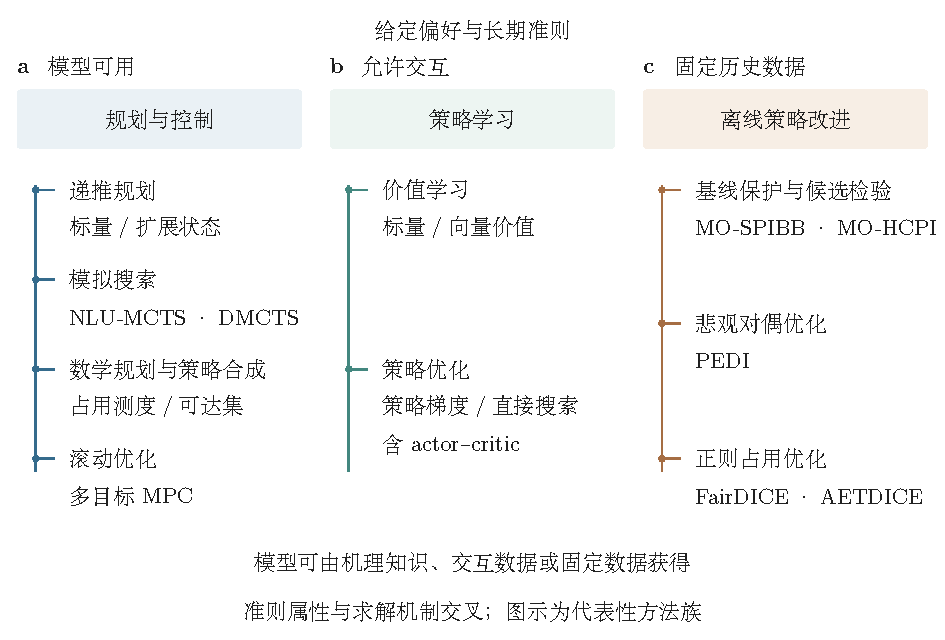
\includegraphics{figures/solver_taxonomy.pdf}
\caption{不同信息条件下的代表性求解机制。三组对应第~\ref{sec:solving-model}--\ref{sec:solving-offline}~节，允许交叉组合，且不构成穷尽分类。MO-SPIBB 与 MO-HCPI 分别采用基线保护约束和候选策略的统计检验\cite{satija2021mospibb}；PEDI 结合对偶更新与悲观估计\cite{wu2021pedi}；FairDICE 与 AETDICE 优化带分布正则项的占用测度，后者在增广状态中处理累计结果变换\cite{kim2025fairdice,kim2026aetdice}。AETDICE 为预印本方法，具体准则和保证条件见正文。}
\label{fig:solver-taxonomy}
\end{figure}

\subsection{模型可用条件下的规划与控制}\label{sec:solving-model}

模型可用时，可以依据状态转移和回报机制预测候选决策的长期影响。显式动力学方程便于构造递推关系、约束条件和数值优化问题；只提供轨迹生成能力的模拟器则适合通过搜索或抽样估计候选策略的长期表现。两种情形下，求解过程都要保留第~\ref{sec:structure}~章所要求的状态信息、价值表示和策略类别。

对于固定线性偏好，或本身就是阶段效用累积的准则，状态满足 Markov 条件时可以直接采用标量动态规划或相应的控制方法。这类规划得到的是执行时根据状态作出反应的闭环策略，与只优化一条固定动作序列的开环规划不同。

累计结果上的非线性 ESR 要求规划保留已实现的结果。NLU-MCTS 将实际执行中已累计的回报与树内搜索及随机 rollout 获得的未来回报按同一折扣基准相加，再对完整结果施加效用函数；反向传播的是这一完整结果的效用，候选动作的期望效用由访问计数估计\cite{hayes2023}。DMCTS 在同一评价结构下维护期望效用的 bootstrap 近似后验，并用 Thompson 采样选择搜索动作。两种方法分别以上置信探索和后验采样分配模拟预算，评价对象都是原 ESR；DMCTS 的后验描述的是期望效用估计的不确定性，并不保存完整的多维回报分布。它们需要能够反复模拟后续过程的模型，搜索预算、rollout 策略和模型误差共同决定最终的动作选择。

扩展状态上的近似动态规划给出了另一条路线。Peng 等在有限状态、有限动作、确定有界向量回报及一致连续效用下，以累计回报网格近似扩展状态，利用连续模 $\delta_\epsilon$ 将回报近似误差转化为效用误差\cite{peng2025esr}：若 $\|\mathbf x-\mathbf y\|_1<\delta_\epsilon$ 时有 $|u(\mathbf x)-u(\mathbf y)|<\epsilon$，有限时域近似动态规划达到 $\epsilon$ 最优，计算复杂度为
\begin{equation}
O\!\left(|\mathcal S|^2|\mathcal A|\left(\frac{mT^2}{\delta_\epsilon}\right)^m\right).
\end{equation}
目标维数以指数方式进入网格规模，时域和精度要求也会抬高代价，无限折扣时域还需额外控制截断误差。这说明，恢复递推结构并不等于求解代价低。一致连续性不要求效用可微，但排除了不连续的阈值效用。

优先级规划通过逐层限制后续决策来保留严格优先关系，而不依赖一个足够大的补偿权重。Wray 等的 LMDP 允许为不同状态分区规定不同的目标顺序，每一级价值迭代完成后，只把相应 $Q$ 值距最优值不超过局部容差的动作传给下一目标\cite{wray2015lmdp}。在无限折扣问题中，局部容差 $\eta_i=(1-\gamma)\delta_i$ 控制其向长期允许损失 $\delta_i$ 的累积；不同分区之间存在循环依赖时，整体收敛还依赖论文给出的分区条件。容差为零与允许高优先级目标让步，对应的是两种不同的决策要求。

部分可观测情形下，同样的思路转移到信念空间。LPOMDP 对所有信念使用同一优先顺序，先按高优先级价值限制每个信念下的可行动作，再进行低优先级备份\cite{wray2015lpomdp}。精确 LVI 保留相应的 $\alpha$ 向量组合，LPBVI 只在采样信念上更新以减少计算。近似价值误差会影响哪些动作被保留或删除，因此需要与容差预算一起处理。

概率阈值和长期平均要求可以直接写成策略合成查询。Brázdil 等用线性约束刻画长期平均多目标问题的可达回报集合，并构造实现相应结果的策略\cite{brazdil2014}。Forejt 等将多目标可达概率与期望总奖励约束化为一系列加权问题：每次求得策略后记录其各目标表现，再用分离超平面选择下一组权重，从内外两侧逼近可达结果集合\cite{forejt2012pareto}。这种查询既能判断给定阈值是否可实现，也能近似给出取舍边界；有限时界要求通过相应时域的价值迭代处理，无界奖励则要求奖励有限并满足相应的符号条件。

Quatmann 和 Katoen 进一步把期望长期平均奖励与期望总奖励的组合纳入多目标模型检验，并扩展到包含连续时间行为的 Markov 自动机\cite{quatmann2021longrun}。算法在允许策略随机化的可达集合上维护
\begin{equation}
\operatorname{downconv}(\mathcal P)\subseteq\mathcal C\subseteq
\bigcap_j\{\mathbf x:\mathbf w_j^\top\mathbf x\leq v_j\},
\end{equation}
其中 $\mathcal P$ 是已实现的期望结果向量，$\mathcal C$ 为逐分量向下闭的可达集合，$v_j$ 是相应加权问题的上界。目标阈值落入内部集合即可实现，超出外部界即不可实现，介于两者之间时继续细化。求解加权子问题时，长期平均部分利用最大端分量内的长期行为，并在商模型中与总奖励部分衔接。该分析要求各目标的上确界有限，混合总奖励还要求端分量内符号一致；它处理的是多个期望准则，不涉及 ESR 或逐轨迹同时达标。

对于具有显式动力学和约束的任务，模型预测控制通过重复求解有限预测时域问题并执行当前动作，实现滚动优化与反馈控制。多目标情形不仅要求得 Pareto 控制序列，还要规定相邻时刻如何在这些序列中选择。设系统动力学为 $x_{t+1}=f(x_t,u_t)$，目标 $i$ 的阶段成本和终端代价分别为 $\ell_i$ 和 $F_i$。Grüne 和 Stieler 的一种构造使用共同的局部终端反馈 $\kappa$，要求每个终端代价满足 $F_i(f(x,\kappa(x)))+\ell_i(x,\kappa(x))\leq F_i(x)$，并在下一时刻选择不劣于移位延续序列的候选解\cite{gruene2019}。在终端不变性、相关 Pareto 集的外部稳定性等条件下，该机制保持可行性，并得到各目标闭环成本上界
\begin{equation}
J_i^\infty(x_0,\mu_N)
\leq J_i^N(x_0,\mathbf u_0^\star),\qquad \forall i,
\end{equation}
其中 $\mu_N$ 是滚动优化形成的闭环控制律，右侧为初始所选预测控制序列的含终端代价成本。Pareto 集的外部稳定性指每个可行成本向量都存在逐分量不劣的 Pareto 向量。若阶段成本之和相对于共同平衡点正定，闭环轨迹还会收敛。这些闭环性质来自选择规则与终端设计的配合；在预测时域内任选一个 Pareto 解得不到这些性质，也不等于原偏好下的无限时域最优策略。

显式多目标 MPC 把重复优化的主要计算移到运行之前。Bemporad 和 Muñoz de la Peña 针对线性动力学，将特定凸分段仿射代价或一个二次目标与其余分段仿射目标的控制问题写成多参数规划，预先构造关于状态和目标权重的分段仿射控制解\cite{bemporad2009mompc}。在线选择权重时还须满足由上一时刻移位序列形成的价值下降约束，稳定性依赖各目标的正定性、共同终端反馈和终端不变性。该方法允许目标权重随状态变化，但为维持稳定可能修正权重，因此实际执行的控制律与最初希望表达的取舍会有差别。

在非线性系统中，Hernández Castellanos 等针对初始状态不确定构建离线控制序列库，利用问题对称性减少需预计算的参数维数，在线阶段插值获得候选，再用参考点优化修正控制序列\cite{hernandez2020explicit}。这一机制把大规模前沿搜索放在离线阶段，在线只针对当前给定偏好做局部求解，修正阶段同时处理不确定性与可行约束。论文的实验针对规定的初始条件不确定集合和汽车机动仿真。

模型方法的实际表现还取决于模型质量、预测时域和数值求解精度。模型偏差影响动作后果的估计，有限预测时域截断远期影响，数值优化引入近似误差；对于数据驱动模型，策略还可能偏向模型误差较大的状态区域。因此，这类方法需要同时报告模型预测性能和闭环策略表现，并说明预测时域、终端价值、约束软化和模型近似各自的作用。

\subsection{允许环境交互条件下的策略学习}\label{sec:solving-online}

准确模型未知但允许交互时，可以用新增的状态、动作和回报样本学习价值函数、环境模型或参数化策略。固定线性偏好与期望可加回报下，先将回报标量化，再采用单目标学习方法即可。需要保留多个目标的信息时，可以学习向量价值，在动作选择或策略更新阶段再引入给定偏好。策略梯度、策略搜索和进化优化则直接以完整策略为优化对象，不依赖局部 Bellman 分解，但要面对长期回报估计方差、探索效率和约束满足等问题\cite{hayes2022}。无论采用哪种表示，学习目标都要与 SER、ESR、优先级或约束结构对应。

非线性 SER 的策略更新需要在整体期望结果处计算目标取舍。设参数化策略为 $\pi_\theta$，固定初始状态分布下的期望累计回报向量为 $\mathbf v(\theta)=\mathbb E_{\pi_\theta}[\mathbf G]$。当效用与期望回报均可微时，由链式法则得
\begin{equation}
\nabla_\theta u_p(\mathbf v(\theta))
=\sum_{i=1}^{m}
\partial_i u_p(\mathbf v(\theta))\,
\nabla_\theta v_i(\theta).
\end{equation}
因此，可以分别估计各目标的策略梯度，再用当前期望结果处的边际效用组合更新方向。这些系数随策略表现变化，计算位置也不同于对每一步即时回报施加非线性效用。Agarwal 等将这一机制用于非线性多目标学习，为每个目标配置 critic 估计价值和优势\cite{agarwal2022nonlinear}。该研究的理论对象是凹、Lipschitz 效用作用于长期平均回报向量的问题：模型方法通过后验采样获得转移模型，在占用测度流约束下求解凹效用最大化，学习保证依赖有限状态动作、有限直径及平稳策略诱导的不可约性；深度 actor--critic 版本则由实验支持。

这类更新还隐含一种不同于回报方差的估计误差。即使 $\widehat{\mathbf v}$ 是期望回报的无偏估计，代入非线性边际效用后，$\mathbb E[\partial_i u_p(\widehat{\mathbf v})]$ 一般也不等于 $\partial_i u_p(\mathbf v)$。Ganesh 和 Aggarwal 的 2026 年预印本针对折扣凹 SER，用多层 Monte Carlo 估计控制这一代入偏差，并结合自然策略梯度更新\cite{ganesh2026bias}。在奖励有界、效用偏导 Lipschitz、策略对数梯度有界且 Lipschitz、Fisher 信息矩阵一致正定等条件下，论文得到 $\widetilde O(\epsilon^{-2})$ 的期望样本复杂度，平均效用差中仍含策略类与兼容函数逼近造成的误差项；若效用满足相应的二阶平滑条件，普通自然策略梯度也能达到同阶结果。由此看，非线性 SER 的样本效率同时受效用平滑性和策略表示条件影响，而不只取决于各目标价值估计的精度。

凹 SER 还可以放到一般效用强化学习的框架中理解。定义折扣占用测度
\begin{equation}
\lambda^\pi(s,a)=\mathbb E_\pi\!\left[\sum_{t\geq0}\gamma^t\mathbf1_{\{S_t=s,A_t=a\}}\right].
\end{equation}
各目标的期望回报是 $\lambda^\pi$ 的线性函数，凹效用 $u(\mathbf v^\pi)$ 因而可以写成占用测度上的凹泛函 $F(\lambda^\pi)$。Zhang 等通过效用的 Fenchel 对偶，将相应策略梯度的估计转化为随机鞍点问题，并利用占用测度中的隐藏凸性分析策略搜索\cite{zhang2020general}。在有限状态动作、初始分布全支持，以及占用测度映射、逆映射和平滑性满足相应条件时，精确梯度迭代具有全局性能收敛界。Barakat 等进一步建立一般凹效用下的梯度支配关系，并通过最大似然估计占用测度，使估计复杂度与所用函数类的参数维数相关\cite{barakat2025general}。其大规模离散问题分析要求占用测度可实现、策略得分及效用梯度有界且平滑，以及参数化保持占用测度的局部可逆结构；可实现性不成立时会留下函数逼近误差。两项工作的全局保证都来自期望回报或占用测度中的结构，而不是策略梯度本身。

公平性准则是非线性 SER 的具体例子。Siddique 等采用广义 Gini 福利函数：先将各目标的期望回报从小到大排序，再以递减的正权重加权，使较差目标获得更大的边际关注\cite{siddique2020fair}。其策略梯度方法根据当前期望回报的排序组合各目标梯度。论文同时指出，所构造的 GGF-DQN 更新实际优化的是期望中的 Gini 评价下界，与期望结果上的评价并不相同，两种算法之间的差别在于随机性的处理方式，而不只是福利函数本身。

若给定准则直接要求改善最差目标，则问题为
\begin{equation}
\max_\pi\min_{1\leq i\leq m}v_i^\pi
=\max_{\lambda\in\mathcal D}\min_{\mathbf w\in\Delta_m}
\sum_{i=1}^m w_i\sum_{s,a}\lambda(s,a)r_i(s,a),
\end{equation}
其中 $\mathcal D$ 是满足折扣流平衡条件的非负占用测度集合。Park 等利用这一结构构造线性规划及其对偶，并以熵正则化消除从对偶最优权重恢复策略时的歧义\cite{park2024maxmin}：只求出一个最优权重、再任选该权重下的确定性最优动作，可能得到最差目标表现为零的策略，最大最小准则仍可能需要随机化。Byeon 等将正则化问题写成策略学习者与目标权重对手之间的零和博弈，以自然策略梯度和镜像下降构成单循环更新\cite{byeon2025maxmin}。其最后迭代收敛分析针对表格 softmax 策略、规定的正则化和步长，近似评价会留下与评价误差相关的邻域，深度 PPO 及自适应正则化版本由实验支持。这里学习到的权重是固定 max-min 准则的求解变量，不是从数据中推断的用户偏好。

多目标梯度方法的保证对象也各不相同。Zhou 等的 MOAC 通过估计共同改进方向，给出折扣和平均回报情形下的有限时间 Pareto 驻点分析\cite{zhou2024moac}。Pareto 驻点表示不存在各目标共同改善的局部方向，与前述凹效用的全局性能界、max-min 正则化博弈的收敛对象含义不同，也不说明某个给定效用已达到全局最优。

非线性 ESR 的学习需要反映效用作用于累计结果这一特点。Reymond 等用多维回报分布构造 critic，把未来回报与已累计结果一起代入效用函数，形成与 ESR 对应的策略更新\cite{reymond2023}。后续研究把分布价值表示用于具体任务，例如基础设施维护中成本与风险的权衡\cite{remmerden2025}。这类方法的关键在于价值表示能提供计算长期效用所需的信息，是否需要完整回报分布取决于具体准则。它与 SER 在均值向量处组合梯度的机制不同：在非线性效用下，逐轨迹结果及其相依关系会影响期望效用。

Cai 等给出另一种保留完整累计效用的在线求解方式\cite{cai2023dpmorl}。在有限时域、$\gamma>0$ 时，把累计回报 $\mathbf c_t$ 和时间加入状态，并构造增量奖励
\begin{equation}
\rho_t=\gamma^{-t}\bigl[u(\mathbf c_{t+1})-u(\mathbf c_t)\bigr],
\qquad
\sum_{t=0}^{T-1}\gamma^t\rho_t=u(\mathbf c_T)-u(\mathbf0).
\end{equation}
右侧与原完整结果效用只差一个常数，因此在扩展信息可用时，标量奖励学习器就能优化原 ESR。等价变换本身不保证 PPO 或 SAC 找到全局最优策略。其 DPMORL 框架还生成多样的单调效用函数并分别训练策略，为分布偏好保留候选，但有限个效用并不覆盖全部单调效用。

词典序学习需要在优化低优先级目标时保住高优先级表现。Skalse 等的价值学习方法按优先级逐层缩小可选动作集合，只保留 $Q$ 值距当前最优值不超过容差的动作，后续目标的备份和选择都限制在这一集合内\cite{skalse2022}。表格收敛结果要求有限状态动作、有界奖励、折扣因子小于 $1$ 或几乎必然终止、所有状态动作对被无限访问，学习率满足随机逼近条件，且容差小于相关非零价值间隙。策略梯度版本通过不同时间尺度的更新和高优先级性能约束实现分层优化。容差、价值估计误差与更新尺度共同决定优先级能否保住，表格情形的收敛结果不覆盖深度函数逼近。期望累计成本约束则把可接受性作为独立的可行域处理，例如 Achiam 等的约束策略优化\cite{achiam2017}，它与词典序的逐层排序承担不同作用。

Abdolmaleki 等的 MO-MPO 在动作分布空间组织多目标更新\cite{abdolmaleki2020mompo}。它为每个目标构造相对于当前策略受 KL 限制的改善动作分布，再通过监督拟合合成单一参数化策略，每个目标允许的 KL 变化量表示其对更新的相对影响。这一接口减弱了奖励尺度对偏好设置的影响，但 KL 参数并不对应某个预先给定效用中的权重。用 MO-MPO 求解给定的效用、阈值或风险要求时，需要说明接口与原准则如何对应，并按原准则评价结果；动作分布的融合也不提供 ESR 所需的累计结果信息。

允许交互的好处是可以主动采集新的决策数据，改善对相关状态与动作的估计；代价是探索本身消耗时间、资源，并可能带来安全风险。对于有安全约束的任务，训练阶段的约束违反和最终部署策略的约束表现应分别记录\cite{skalse2022,achiam2017}。训练主要在仿真器中进行时，还要区分仿真样本效率与真实系统的数据成本；若学习过程同时估计模型并据此规划，实际采集的数据与模型生成的数据也应分开说明。

\subsection{固定历史数据条件下的策略学习}\label{sec:solving-offline}

离线条件下，策略只能用预先收集的历史数据训练，无法通过新的交互验证或补充当前策略所需的信息。离线求解首先要回答两个问题：数据记录了哪些变量，行为策略覆盖了哪些状态、动作和长期结果。

第一个问题决定数据能否重建原长期准则。数据保存了原始多维回报时，只要环境机制与目标定义不变，就可以按任意固定权重重新构造标量回报；若只保存了某一历史权重下的标量奖励，各目标分量已被压缩，可分析的偏好范围随之受限。阶段效用累积需要逐阶段回报，或足以恢复阶段效用的信息；累计结果上的非线性 ESR 需要轨迹关联信息，至少要能重建累计量、事件和约束；非线性 SER 则需要据此估计候选策略的期望回报向量。

第二个问题决定策略估计的可靠性。候选策略频繁选择数据中很少出现的动作时，其价值估计主要依赖函数逼近和分布外外推。单目标离线强化学习常用保守价值估计、行为约束或不确定性建模控制外推误差\cite{kumar2020}；多目标问题还需要明确这些机制保护的是加权总价值、各目标表现，还是原有的可接受性条件。较强的行为约束限制了外推，也限制了策略超越历史行为的空间；偏好变化则会改变需要改进的行为区域。

线性偏好下，可以显式限制离线改进的幅度，使各目标都不差于基线。MO-SPIBB 在有限状态动作、有界奖励及已知行为基线 $\pi_b$ 的条件下优化正线性权重下的价值，并要求策略在估计不确定性较大的动作上接近基线\cite{satija2021mospibb}。其 Soft-SPIBB 约束为 $\sum_a e(s,a)|\pi(a\mid s)-\pi_b(a\mid s)|\leq\epsilon$，其中 $e(s,a)$ 是由日志数据得到的误差界；算法还加入各目标的基线优势约束，并在每个状态求解线性规划。在概率至少为 $1-\delta$ 的估计事件上，各目标真实价值满足
\begin{equation}
V_i^\pi(s)-V_i^{\pi_b}(s)
\geq-\frac{\epsilon V_{\max}}{1-\gamma},\qquad i=1,\ldots,m,
\end{equation}
其中 $V_{\max}$ 为价值幅度上界。这是一种允许统计误差的逐目标基线保护，并非逐条轨迹的物理安全保证。同一研究中的 MO-HCPI 使用独立的训练与安全检验数据，通过各目标的重要性加权下置信界联合筛选候选策略。两者分别代表优化约束和事后统计检验两条路径。

非线性 SER 与期望结果约束可以通过对偶化和悲观估计共同处理。PEDI 研究有限时域成本问题 $\min_\pi g(\mathbf V^\pi_1)$，并要求期望累计成本向量位于给定目标集内\cite{wu2021pedi}。其中 $g$ 为凸、逐坐标单调不减且 Lipschitz 的函数，目标集为满足几何 Slater 条件的非空闭凸下集。算法利用凸共轭把非线性成本和目标集距离惩罚转化为一系列线性成本问题，交替执行对偶变量更新与悲观价值迭代；由于目标是成本最小化，悲观性体现为在成本估计中加入不确定性惩罚。最终策略在每次执行开始时随机选取一个迭代策略并全程执行，以实现迭代价值的平均。性能差距与约束违反界都含有沿最优策略轨迹累积的数据不确定性，因此不要求全空间统一覆盖，但最优行为的支持不足时误差界会很大。这些保证针对期望成本。

占用测度优化提供了处理非线性长期效用的另一条路径。FairDICE 将各目标期望回报的严格凹福利总和与相对于数据占用分布的 $f$ 散度正则化共同优化，并以占用流约束保证策略一致性\cite{kim2025fairdice}。其对偶变量对应当前福利目标的边际取舍；在最优对偶权重处，正则化非线性问题与相应的正则化线性问题等价。这里的权重由已给定福利函数的优化产生，不是学习到的决策者偏好。AETDICE 将评价形式扩展为 $\mathcal G(\mathbb E[\mathcal F(\mathbf G^\pi)])$，在有限时域中把已累计回报与时间加入状态，利用变换 $\mathcal F$ 的增量奖励建立占用测度优化，从而覆盖 SER、ESR 及其组合\cite{kim2026aetdice}。外层 $\mathcal G$ 为线性时，可以得到与相应可加目标的等价表示；一般分析还依赖外层凹性、变换平滑性及正则项的严格凸性。该方法要求数据在每个可达的增广状态、动作和时刻上具有正占用密度，这比普通状态动作上的支持要求更强。

上述方法分别用逐目标基线保护、悲观对偶优化和占用测度正则化控制离线改进，优化对象和保证范围各不相同。约束、尾部风险和达标概率需要与原准则匹配的估计，主目标上的保守性推不出它们的表现。离线求解前应分别检查两件事：数据能否重建长期准则，以及数据是否覆盖目标策略的决策区域。这两项条件互不替代，增加同类样本也无法弥补记录内容的缺失。

\subsection{跨偏好的计算与数据复用}\label{sec:solving-reuse}

偏好在求解时已经给定，但不同偏好之间仍可以共享数据和计算。常见的组织方式有三种：针对当前偏好独立求解；预先构建覆盖多种偏好的候选策略集合；训练以偏好或目标结果为条件输入的统一策略。三种方式都能服务于给定偏好决策，区别在于训练成本、表示范围和泛化要求\cite{vamplew2011}。本节按信息条件介绍后两种方式，最后讨论非线性效用下的候选覆盖。

图~\ref{fig:preference-reuse}~对照了三种方式从给定偏好到执行策略的接口与共享对象。

\begin{figure}[H]
\centering
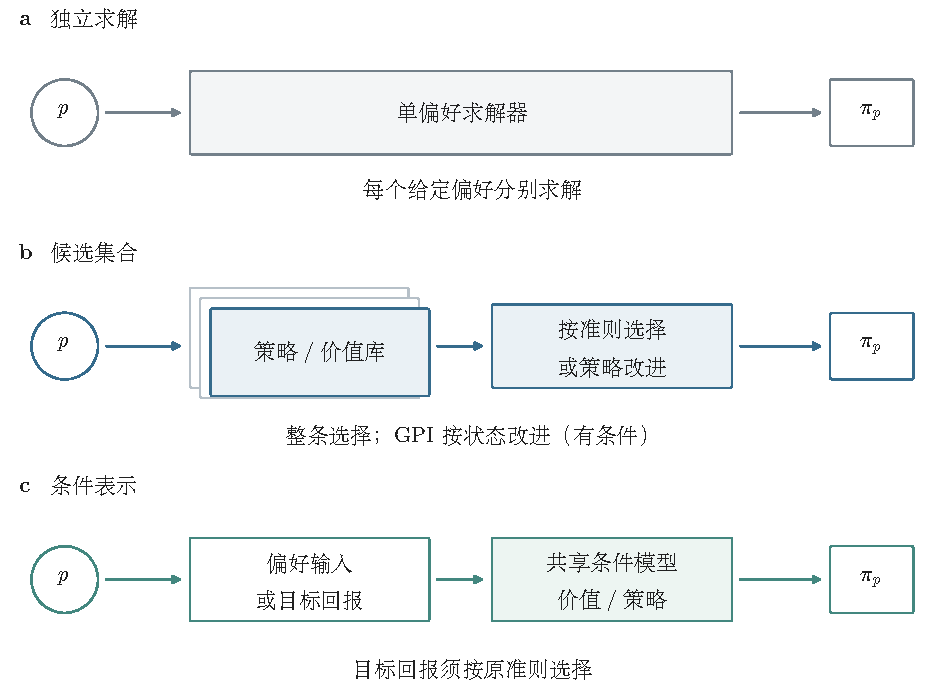
\includegraphics{figures/preference_reuse.pdf}
\caption{面向多个给定偏好的求解组织方式。独立求解为每个偏好分别计算策略；候选集合复用已有策略及其评价；条件表示共享模型参数。整条策略选择与逐状态的广义策略改进（GPI）不同，后者的性能性质依赖回报结构与评价精度等条件\cite{barreto2017sf}。条件价值需经动作选择形成策略；目标回报条件模型须先按原准则确定目标，不能把目标回报等同于偏好权重\cite{reymond2022pcn,zhu2023}。三种组织方式可以组合，图中不比较性能或计算成本。}
\label{fig:preference-reuse}
\end{figure}

\subsubsection{模型可用时的候选集合规划}

共享多个线性偏好的规划可以在算法内部或外部组织。内部方法直接把标量价值替换为候选向量集合：凸包价值迭代（CHVI）在状态动作对上保留对某个线性权重最优的向量，通过后继集合的加权组合与凸包剪枝完成备份\cite{barrett2008}。与保留全部 Pareto 向量相比，它只保存线性偏好所需的凸覆盖信息。

环境随机时，候选集合的递推要组合不同后继状态上的后续选择。Chen 等以有限状态动作、非负成本的多目标随机最短路径问题为例，采用向量集合价值迭代，并通过启发式搜索减少需要更新的状态\cite{chen2023mossp}。设 $\mathcal V_k(s)$ 表示状态 $s$ 的候选期望成本向量集合，其更新可写为
\begin{equation}
\begin{aligned}
\mathcal Q_{k+1}(s,a)
&=\{\mathbf c(s,a)\}\oplus
\bigoplus_{s'}P(s'\mid s,a)\mathcal V_k(s'),\\
\mathcal V_{k+1}(s)
&=\operatorname{CCS}\!\left(\bigcup_a\mathcal Q_{k+1}(s,a)\right),
\end{aligned}
\end{equation}
其中 $\oplus$ 为向量集合的 Minkowski 和，$\operatorname{CCS}$ 保留支持线性成本权衡的凸覆盖信息。这里采用到达目标即终止的无折扣成本，目标状态 $g$ 的终端集合为 $\mathcal V_k(g)=\{\mathbf 0\}$。不同后继状态可以对应不同的后续决策，因此期望运算需要组合各后继状态的候选向量。MOLAO* 在部分解图上扩展状态并更新其祖先，MOLRTDP 通过试运行和残差检查逐步标记已求解状态，二者都要处理多个不可比较的候选动作。收敛分析要求适当的可达性条件和可采纳启发式，并需排除不能以概率 $1$ 到达目标的策略；论文用适当策略成本的已知向量上界识别这类不适当策略。这些结果针对线性成本权衡下的凸覆盖。

集合值递推还要保证组合出来的尾部选择能由允许的策略实现。Mifrani 对 White 的早期向量 Bellman 扩展给出有限时域反例：分别从不同后继状态选取候选尾部价值并求加权和，所得向量未必对应同一条确定性 Markov 策略，因为不同分支随后汇合时，可能要求该策略在同一状态与时刻采取不同动作\cite{mifrani2025bellman}。在该研究的模型中，确定性转移，或允许策略利用已达状态的历史，可以恢复集合方程的可实现性。CON-MODP 处理的正是这一问题：它同时存储价值与策略，对只在当前扩展状态出现冲突的候选强制采用同一动作并重新评价，其收敛结果针对确定性转移的无限时域折扣多目标 MDP\cite{wiering2007conmodp}。因此，对向量价值集合做备份时，除了数值上的支配关系，还要说明集合覆盖的策略类别，以及后继策略的组合是否仍属于该类别。

精确剪枝通常需要反复求解线性规划，检验某一候选是否存在能使其优于其余候选的权重或信念。BLP 利用相邻价值迭代中这些线性规划的相似性，把上一轮相似问题中决定最优解的约束映射到当前候选集合作为初始约束，再逐步加入违反的约束，直到完成原问题的检查\cite{roijers2018bootstrap}。它减少的是重复求解的工作量，剪枝检验本身照常完成，这与直接截断候选集合、以覆盖精度换速度的近似机制不同。

外部方法保留单目标求解器，通过选择权重逐步构建覆盖。AOLS 利用当前标量化价值包络的分片线性凸结构，在潜在改进较大的角点权重处调用求解器，并根据新增向量重新计算角点与误差界\cite{roijers2014aols}。底层求解器具有已知的相对近似保证时，该误差可以用来构造近似凸覆盖；底层若只是没有误差证书的启发式规划器，就得不到同样的覆盖保证。对于给定偏好问题，这类多偏好规划的作用是预先复用计算；如果只需处理一个固定偏好，应比较额外覆盖成本与直接求解的成本。

不完全观测会改变规划所需的状态。对于转移与观测模型已知的多目标 POMDP，OLSAR 将单目标 POMDP 的 $\alpha$ 向量扩展为保留各目标价值的 $\alpha$ 矩阵；给定信念 $b$ 和权重 $\mathbf w$，候选矩阵 $A$ 的标量价值为 $b^{\mathsf T}A\mathbf w$\cite{roijers2015olsar}。外层乐观线性支持依据当前凸覆盖的潜在改进选择待求解权重，内层点基规划用先前得到的矩阵初始化价值下界，从而避免从头规划，也减少额外的策略评价。近似覆盖保证继承底层标量 POMDP 求解器的误差；采用点基方法时，该误差还取决于采样信念对信念空间的覆盖密度，矩阵复用本身主要改善计算时间。与 OLSAR 按线性权重构建覆盖不同，第~\ref{sec:solving-model}~节的 LPOMDP 在信念空间中共享的是保持优先级的动作限制，两者不能通过更换权重输入相互替代。

\subsubsection{交互学习中的策略库与条件策略}

策略库方法首先共享已有策略及其评价。Natarajan 和 Tadepalli 在加权平均回报问题中缓存有限个策略及其向量评价，新权重给定后选择已有策略继续改进\cite{natarajan2005}。DOL 将外循环乐观线性支持与向量输出的深度 Q 学习结合，比较了复用全部网络参数与只保留特征层、重新训练输出层两种做法\cite{mossalam2016dol}。复用收益来自已有表示对后续偏好求解的初始化；神经子求解器的近似误差会进入覆盖结果，外循环的理论性质并不延伸到深度训练过程。

策略集合需要解决多个候选价值如何共同学习，以及执行时如何恢复所选策略。Pareto Q-learning 将即时回报的均值与后续非支配价值集合分开保存，避免在不断变化的两个向量集合之间建立不稳定的一一更新关系\cite{vanmoffaert2014pql}。确定性转移下，动作价值集合由即时均值加上折扣后的后继候选集合构成；随机转移扩展则按观测到的转移频率组合不同后继状态的向量集合。学习阶段可以用超体积、集合基数或支配关系引导探索；执行阶段则要先选定一个目标期望回报向量并持续跟踪对应策略，而不是在每个状态任选一个局部非支配动作。该方法针对回合式任务学习确定性非平稳候选策略，论文没有给出正式的收敛证明，其价值集合也不是 ESR 所需的回报分布表示。

在共享动力学、只有回报权衡变化的任务中，后继特征为复用提供了显式分解。若条件期望即时回报满足 $r_{\mathbf w}(s,a,s')=\boldsymbol\phi(s,a,s')^\top\mathbf w$，则
\begin{equation}
\begin{aligned}
Q_{\mathbf w}^{\pi}(s,a)
&=\boldsymbol\psi^\pi(s,a)^\top\mathbf w,\\
\boldsymbol\psi^\pi(s,a)
&=\mathbb E_\pi\!\left[\sum_{t\geq0}\gamma^t\boldsymbol\phi(S_t,A_t,S_{t+1})\mid S_0=s,A_0=a\right].
\end{aligned}
\end{equation}
Barreto 等据此在新权重下直接重评既有策略，再进行广义策略改进\cite{barreto2017sf}。Borsa 等的通用后继特征近似进一步把策略的任务编码作为条件输入，使价值表示能在已学策略之间泛化\cite{borsa2019usfa}。前者复用回报权重，后者复用策略表示，两者都以共享动力学、线性回报表示和足够准确的评价为前提。

给定新偏好后，广义策略改进（GPI）用当前权重评价库 $\Pi$ 中每个策略的向量动作价值，再在动作和策略两个维度上选择：
\begin{equation}
\pi_{\mathrm{GPI}}(s;\mathbf w)
\in\arg\max_a\max_{\pi\in\Pi}
\mathbf w^{\mathsf T}\mathbf Q^\pi(s,a).
\end{equation}
在固定线性偏好、折扣可加回报及准确策略评价下，所得策略至少不劣于库中任一策略\cite{alegre2026}。与整条选用库中某个策略不同，改进策略可以逐状态利用不同候选策略的后续价值。Alegre 等进一步以 GPI 能带来的价值改进决定训练哪些权重，并用相应误差确定生成和使用模型样本的优先级。GPI-LS 的覆盖保证要求单偏好求解器达到最优或规定的近似精度；GPI-PD 学习下一状态与完整向量奖励的联合模型，使同一模型服务于多个权重；其不确定性感知扩展用价值估计的置信下界抑制高估动作，在下界有效时给出相对于库中最好策略的性能余量。这些保证建立在线性组合、候选覆盖和估计误差之上。

多个偏好也可以作为相关子问题，在策略群体中共享搜索信息。MORL/D 将偏好采样、经验池、邻域协作、策略改进与外部档案组织为可组合的求解框架\cite{felten2024decomposition}。PGMORL 维护策略群体，依据历史改进数据预测不同训练方向的收益，选择策略和权重继续训练，并通过 Pareto 分析和插值扩展候选\cite{xu2020pgmorl}。与每个权重从头训练相比，这些方法把计算分配和经验共享纳入复用机制，其覆盖质量和插值效果由实验评估，没有给定偏好下的效用误差保证。

连续候选集也可以不以偏好权重为输入。Parisi 等学习从低维变量到策略参数的流形，使其在目标空间中的像逼近 Pareto 前沿\cite{parisi2016manifold}；后续工作在每次执行开始时探索策略参数，并以重要性采样复用历史执行数据\cite{parisi2017reuse}。使用时仍需依据原效用在流形可表示的候选中选择，前沿质量指标的优化也不等同于对每个给定效用取得最优。

条件价值网络则用一个网络代替显式存储的策略集合。Abels 等把线性权重作为多目标价值网络的输入\cite{abels2019}，Envelope 方法更新时在当前权重下同时比较不同动作和其他权重对应的候选向量价值\cite{yang2019}：更新下一状态价值时，选择使 $\mathbf w^{\mathsf T}Q(s',a',\mathbf w')$ 最大的候选向量，而不只在当前权重 $\mathbf w$ 下搜索动作，再把该向量与即时向量回报组成更新目标。这样，其他偏好下已探索到的折中结果也能用于当前偏好的学习。作者在有界价值、折扣因子小于 $1$ 的理想更新设定中，以各权重的标量化价值定义伪距离并分析固定点；实际的深度网络通过有限偏好采样、向量误差与标量化误差的联合训练近似这一更新，理想算子的收敛结论不覆盖这一训练过程。

近期研究进一步处理条件网络中的共享表示和训练冲突。COLA 用与目标无关的潜在动力学表示共享转移知识，并在不同偏好的价值更新发生冲突时限制相互干扰\cite{li2025cola}。$D^3$PO 公开稿分别计算逐目标优势和 PPO 裁剪损失，再按偏好加权，并用动作分布差异正则化抑制条件策略的行为塌缩\cite{ambadkar2026d3po}。Chen 等从无奖励强化学习出发，把其训练目标作为辅助任务，并结合偏好引导探索，以改善不同偏好之间的知识共享\cite{chen2026rewardfree}；训练阶段为多个潜在查询收集可复用信息，回答查询时偏好仍是给定输入，相关实验以 MO-Gymnasium 基准和消融设置检验辅助任务与探索策略的作用。这些工作都在连续控制或标准基准上检验机制，没有给出非线性效用下的覆盖保证。

样本重用方式会改变条件网络实际学到的偏好范围。Bonin 等的近期公开稿研究了以已实现结果方向替换请求偏好的回溯重标记，发现在所测的离策略连续控制任务中，该机制可能使训练集中到少数已访问的偏好区域，并提出混合保留原请求偏好的修正\cite{bonin2026collapse}。结论限于所测算法、目标数和任务；它的启示是，应检查样本复用是否持续覆盖需要回答的偏好查询，而不是只看数据被重复使用的次数。

条件策略中的“偏好一致”也可能指不同的目标。PCRL 将输入参数解释为期望回报方向，通过目标梯度与方向相似性梯度共同更新\cite{yang2025pcrl}。其理论分析给出平滑性、梯度估计及步长等条件下的 Pareto 驻点和相似性驻点，论文也指出驻点未必具有高相似度。回报方向接近输入参数，与最大化同一参数所定义的线性加权效用，是两种需要分别评价的选择规则。

目标回报条件策略提供了不同于价值递推的共享路径。Pareto Conditioned Networks（PCN）把状态、目标剩余回报向量及剩余时域作为输入，把轨迹中实际采取的动作作为监督标签，通过动作分类训练一个能够复现不同结果的网络\cite{reymond2022pcn}。每条新轨迹按各时刻的实际后续回报重新标注；训练期间，算法从已有非支配结果附近提出改进目标，继续与环境交互，并保留不同结果区域的轨迹以维持覆盖。因此，PCN 虽然使用监督更新，整体仍包含主动采集轨迹。部署时输入的是目标结果而非效用权重，要服务于给定偏好，还需依据原效用或可接受性规则选定希望实现的结果，并检验条件策略的实际表现。实验展示了单个网络覆盖非凸折中区域的能力，论文没有给出任意目标回报可达或任意非线性效用最优的理论结论。Vamplew 等的 steering 方法同样以目标点组织非平稳策略学习，并与平稳确定性策略进行实验比较\cite{vamplew2017steering}。这类目标点接口都需要与给定效用或可接受性规则相连；本文只讨论目标已经给定时的求解接口，不讨论用户在学习过程中修改目标的情形。

\subsubsection{固定数据下的偏好复用}

固定数据下，多个偏好可以共享同一批轨迹。Lizotte 等在有限时域、无折扣的多奖励批量学习中，以线性函数拟合各动作的价值，并在权重单纯形上保留分片线性表示\cite{lizotte2012}。在特征矩阵满列秩且采用无正则最小二乘时，省略动作下标，某一阶段的回归系数可写为
\begin{equation}
\widehat{\boldsymbol\beta}_t(\mathbf w)
=(\Phi_t^{\mathsf T}\Phi_t)^{-1}\Phi_t^{\mathsf T}\widehat{\mathbf y}_t(\mathbf w),
\qquad
\widehat y_{t,n}(\mathbf w)
=\mathbf w^{\mathsf T}\mathbf r_{t,n}
+\widehat V_{t+1}(s_{t+1,n},\mathbf w),
\end{equation}
其中 $\Phi_t$ 是特征矩阵，$n$ 标识历史样本。终端阶段可以线性组合各基奖励的拟合系数；此前阶段的最优动作随权重变化，回归目标需要依据各样本的权重分区共同细分，三目标情形则通过单纯形三角剖分组织这些分片。这种复用依赖回归与价值包络的结构，分片数会随时域和目标维数增长，只训练偏好端点再插值得不到全部策略。

MOFQI 不显式维护单纯形上的分片，而是把固定偏好参数作为价值函数的输入。它将单目标拟合 $Q$ 迭代扩展到状态、动作与线性权重的联合空间，在一次训练中共享不同权重下的回归\cite{castelletti2012mofqi,castelletti2013water}。在成本最小化记号下，备份仍针对同一权重计算后续价值，即以 $\mathbf w^{\mathsf T}\mathbf c+\gamma\min_{a'}\widehat Q_{k-1}(s',a',\mathbf w)$ 构造回归目标；同一环境转移可以配上多个采样权重，但权重在一次序贯问题中保持不变。与解析保留分片相比，树回归直接逼近连续偏好域，减轻了显式分区的存储负担，精度则取决于样本、权重采样和函数逼近。

对于带偏好标签的多目标示范，PEDA 以偏好和向量剩余回报为条件，通过 Decision Transformer 或回报条件监督学习生成动作\cite{zhu2023}。训练数据按各目标尺度归一化，动作损失拟合历史轨迹中的行为；部署时要给出与当前偏好匹配、且数据能够支持的目标回报。D4MORL 中不同数据质量与偏好覆盖的设置显示了这些信息条件的影响；其实验指标依据行为策略的参考前沿计算，并不代表相对真实最优前沿的性能。若示范的偏好没有记录，直接模仿全部轨迹会把相互冲突的取舍混进同一行为正则项。PRMORL 用归一化轨迹回报近似行为偏好，根据它与给定权重的相似度筛选示范，并结合表达能力更强的生成策略及偏好条件价值学习\cite{lin2024offline}。这一标签推断只用于筛选历史数据，当前决策者给定的偏好仍是优化输入；轨迹回报提供的是启发式标签。该方法在部署时调整行为正则化强度的阶段使用了新采集的环境轨迹，这部分适应成本应与固定数据训练分开计算。

偏好条件生成方法以轨迹片段为建模对象。MODULI 以偏好和回报为条件生成状态序列，再用逆动力学模型恢复待执行动作；它对目标回报做偏好相关的归一化，并学习沿偏好变化方向调整去噪过程的适配器，把生成从数据覆盖区域引向未覆盖的偏好区域\cite{yuan2025moduli}。DiffMORL 同样采用偏好条件扩散规划，但主要通过离线数据混合增强训练样本，改善对未见偏好的生成表现\cite{xiao2025diffmorl}。前者调整生成时的条件引导，后者增强训练数据，两者都不同于 PEDA 直接监督拟合历史动作。D4MORL 实验支持它们在所测偏好分布上的泛化表现；生成轨迹和扩充的条件标签仍需由实际动力学与回报支持，生成能力本身说明不了未覆盖偏好下的最优性或可行性。

偏好条件方法复用的是数据中已有的行为，不会增加数据中没有观察到的动作后果。因此，第~\ref{sec:solving-offline}~节关于记录内容和数据覆盖的两项检查同样适用于这里，而且需要针对每个待回答的偏好分别进行。

\subsubsection{非线性效用下的候选覆盖}

线性权重下的凸覆盖只保留了均值信息。非线性 ESR 下，Röpke 等研究了多维回报分布之间的支配关系，以及它与期望效用和 Pareto 支配之间的联系\cite{ropke2023}。其分布支配以联合累积分布函数的排序为基础，并要求至少一个目标的边缘分布严格改善。相应的分布未支配集（distributional undominated set，DUS）保留不被其他候选分布支配的策略，它包含期望回报的 Pareto 前沿，也可能保留在期望意义下受支配的策略。凸分布未支配集（convex distributional undominated set，CDUS）进一步检查其他回报分布的混合能否支配某一候选，以缩小集合规模。

这类剪枝的效用保证有明确的范围。该研究对两维回报证明：对于严格单调且满足 $\partial^2u/\partial x_1\partial x_2\leq0$ 的效用，分布支配意味着更高的期望效用，混合支配则保证至少有一个组成分布优于被支配的候选。该交叉导数条件描述的是目标联合取值的偏好结构，与效用的凹性是两回事。联合分布还保留了目标间的依赖；用边缘累积分布函数的乘积代替联合分布，只有在目标独立时才有相应的支配解释。计算中，回报被投影为有限类别分布，使支配检查能在有限支持点上进行；分布精度与候选集合规模都会增加存储和计算代价，额外的集合截断也可能丢掉需要的候选\cite{ropke2023}。因此，只依据期望回报向量筛选 ESR 候选可能丢失有价值的策略，而分布表示与剪枝规则也必须和具体的效用类别相匹配。

对于明确给定的非线性效用族，已有工作直接以原准则性能定义覆盖。Kim 等针对广义 $p$-mean 福利函数，把 max-min、几何平均与算术平均纳入 $p\in[-\infty,1]$ 的同一参数族，并分别给出 SER 和 ESR 两种聚合\cite{kim2025portfolio}。在有限状态动作、固定起点与固定有限时域、逐阶段各目标奖励严格正有界 $0<L\leq r_i\leq U$，且能在同一可行策略集合 $\Pi$ 内求出每个参数 $p$ 下最优策略的条件下，其算法自适应选择参数，构造对整个族都具有 $\alpha$ 乘法近似保证的策略组合；记 $\kappa=U/L$，组合规模上界为 $O(\log\kappa/\log(1/\alpha))$。相邻参数热启动分析还控制了已有最优策略在新参数下的福利损失。这里的组合是供不同效用选择的候选集合，执行时不需要随机混合；用启发式求解器替代最优 oracle 后，近似保证需要相对于该求解器重新解释。这一结果说明，跨偏好复用可以围绕明确的效用族建立性能保证，而不只依靠前沿几何指标描述覆盖。第~\ref{sec:solving-online}~节 DPMORL 生成的多样单调效用也服务于同一目的，但没有相应的覆盖保证。

\subsubsection{复用方法的适用范围}

上述方法共享数据、表示和计算的方式不同：显式价值集合保留多个可比较的结果，条件价值网络共享各偏好下的估计，GPI 利用候选策略的价值做逐状态改进，目标回报条件网络则共享已实现结果与动作之间的映射。策略的组织形式需要与偏好类别、可搜索的策略类别以及数据支持范围相对应。

复用方法的有效范围由训练时覆盖的偏好形式和参数区域决定。线性权重下的凸覆盖和均值信息、非线性 SER 在受限策略类别下的候选保留要求、非线性 ESR 的分布信息要求，三者需要分别分析；允许策略混合时，可达期望回报集合也会改变。参考点、词典序和硬约束可能要求不同的条件输入、排序机制和可接受性检查，只修改一个权重标签并不能让原有网络覆盖这些问题。针对单一偏好的专门求解可以集中模型容量和采样资源；复用方法的收益则应通过覆盖误差、新偏好的追加求解成本和部署计算量来衡量，而不只看平均解集指标。

最后，在不同任务之间切换偏好，与在同一执行过程中改变偏好是两类问题。前者是多个给定偏好问题之间的策略复用；后者会影响已实现累计结果的解释，并可能改变整个长期决策准则。本文关注求解或部署开始时已经确定的偏好，因此把跨偏好方法视为数据与计算的复用机制，不展开偏好获取和执行中偏好变化的问题。

\subsection{结构条件与求解路线的对应}\label{sec:solving-summary}

综合第~\ref{sec:structure}~章的结构分析与本章的方法，求解路线可以按“长期准则---信息表示---策略类别---模型与数据条件”的顺序组织。长期准则决定评价什么，状态与价值表示决定保留哪些信息，策略类别限定可搜索的决策规则，模型与数据条件决定这些信息从何处获得。

表~\ref{tab:solver-routes}~汇总上述对应关系。可等价转化的期望可加准则允许直接调用标量方法；非线性 SER 围绕期望向量或占用测度组织优化，非线性累计结果 ESR 则需保留足以计算完整结果效用的信息。词典序、期望约束和路径概率要求还须保留各自的比较次序或可接受性条件，不能相互代替。实际任务中的这些结构可以组合，具体方法的保证仍以相应的效用、策略、模型和数据假设为前提。

\begin{table}[H]
\centering
\caption{长期准则与模型、数据条件下的求解路线}
\label{tab:solver-routes}
\begingroup
\zihao{5}\songti
\setlength{\tabcolsep}{5pt}
\renewcommand{\arraystretch}{1.18}
\setlength{\reviewtablewidth}{\dimexpr\textwidth-6\tabcolsep\relax}
\begin{tabular}{@{}P{0.25\reviewtablewidth}P{0.25\reviewtablewidth}P{0.25\reviewtablewidth}P{0.25\reviewtablewidth}@{}}
\toprule
准则与关键信息 & 模型可用 & 允许交互 & 固定历史数据 \\
\midrule
期望可加标量准则\newline 固定取舍、Markov 信息 & 标量动态规划\cite{hayes2022}\newline 转移与回报模型 & 标量回报学习\cite{hayes2022}\newline 探索与采样条件 & 重标奖励后学习\cite{zhu2023}\newline 原始回报与行为支持 \\
\addlinespace[7pt]
非线性 SER\newline 期望向量、策略随机化 & 凹效用占用优化\cite{zhang2020general}\newline 有限状态动作等条件 & 整体期望处组合梯度\cite{agarwal2022nonlinear}\newline 区分理论与深度实现 & FairDICE\cite{kim2025fairdice}\newline 凹福利的正则占用优化 \\
\addlinespace[7pt]
非线性累计结果 ESR\newline 累计量、时间、效用信息 & 扩展状态近似规划\cite{peng2025esr}\newline 有限模型、连续效用；或模拟搜索\cite{hayes2023} & 累计状态与效用增量\cite{cai2023dpmorl}\newline 有限时域下保持目标 & AETDICE\cite{kim2026aetdice}\newline 增广状态上的正则优化与数据支持 \\
\addlinespace[7pt]
优先关系\newline 次序、容差、估计误差 & LMDP 逐层限动作\cite{wray2015lmdp}\newline 容差与分区条件 & 词典序价值或策略更新\cite{skalse2022}\newline 充分访问、适当容差 & 本文未作\newline 专门方法比较 \\
\addlinespace[7pt]
期望结果约束\newline 目标、可行域、随机化 & 约束查询与可达集逼近\cite{forejt2012pareto} & CPO\cite{achiam2017}\newline 期望成本约束下的策略更新 & PEDI\cite{wu2021pedi}\newline 凸成本、目标集及数据支持 \\
\addlinespace[7pt]
路径概率或联合达标\newline 事件、记忆、联合信息 & 概率性质合成\cite{etessami2008modelchecking}\newline 可能需记忆与随机化 & 按指定事件评价和更新；本文未作专门比较 & 事件可恢复、策略有支持；均值保护不等于概率保证 \\
\bottomrule
\end{tabular}
\par\vspace{4pt}\raggedright\noindent
注：各行可组合，信息条件也可交叉；完整条件见第~\ref{sec:solving-model}--\ref{sec:solving-offline}~节。标量化仍须匹配时间结构并保留独立约束；ESR 近似规划中的效用要求一致连续。FairDICE、AETDICE 含分布散度正则，AETDICE 为预印本。未列专门方法不表示该方向不存在方法。
\par\endgroup
\end{table}


当多个给定偏好需要依次求解时，第~\ref{sec:solving-reuse}~节的复用方法可以分摊计算和数据成本，但其保证范围受偏好类别、候选覆盖和估计误差的限制。求得策略后，还要检验它是否实现了原定的长期准则，这是下一章讨论策略评价的起点。

% !TeX root = main.tex
\section{策略评价与应用}\label{sec:evaluation}

给定偏好下的策略评价要回到最初定义的长期决策准则，训练损失、内部奖励和解集指标反映的是算法的部分性质，最终要判断的是策略是否实现了预期的目标取舍和约束要求。本章的安排是：先讨论单个策略与策略集合在原准则下的评价；随后考察评价所依赖的信息条件，包括只有历史数据时的离线评价、实验比较规范以及鲁棒性与部署条件；最后结合代表性应用，说明不同层次的实验证据各自能支持哪些结论。

\subsection{单策略在原准则下的评价}\label{sec:eval-criteria}

对于采用实值效用的任务，首先应报告策略在原长期准则下的表现，同时保留各目标的结果，以便分析效用的改善来自哪些目标、为此付出了什么代价。能精确求得最优值时，可以进一步报告最优性差距；只有基线或近似参考解时，结果应表述为相对于该参考的性能差异。严格词典序等非标量比较关系，按原比较规则评价，不额外构造加权总分。

当评价对象为累计回报向量时，SER 与 ESR 对样本的聚合顺序不同。设同一固定策略在相同初始状态分布下独立执行，得到累计回报样本 \(\mathbf G^{(1)},\ldots,\mathbf G^{(N)}\)，两者的估计为
\begin{equation}
\begin{aligned}
\widehat J_{\mathrm{SER}}
&=
u_p\!\left(
\frac{1}{N}
\sum_{n=1}^{N}\mathbf G^{(n)}
\right),\\
\widehat J_{\mathrm{ESR}}
&=
\frac{1}{N}
\sum_{n=1}^{N}
u_p\!\left(\mathbf G^{(n)}\right).
\end{aligned}
\end{equation}
SER 先对回报向量取样本均值再施加效用，ESR 先计算每次执行的效用再取平均，与第~\ref{sec:criteria-stochastic}~节的定义的运算顺序一致\cite{hayes2022}。非线性效用下，SER 的有限样本代入估计有其自身的统计性质，置信区间和误差分析也要按相同的聚合顺序进行。

上式对应以累计回报向量为评价对象的准则。若原目标是阶段效用的期望累积，就先在每条轨迹内按既定时域和折扣累加阶段效用，再对轨迹结果取期望；若准则直接作用于轨迹特征，就先从完整轨迹或相应的充分统计量中计算该特征，再进行评价。路径事件、首次到达时间和累计资源使用等指标同样按各自的定义处理。评价公式由原长期准则决定，而不是由算法的输出形式决定。

满意水平、风险和约束问题，除效用本身外还要报告达标与违反情况。多个目标需要同时满足时，统计联合达标概率；连续约束可以同时报告违反频率和违反幅度。罕见失效或尾部风险的结果，要结合样本规模、评价时域和不确定性估计来解释。

除数值比较外，还可以展示策略的目标分量、主要取舍和结果的不确定性。多目标决策支持的研究已经系统整理了候选解可视化、解集分析和不确定性探索方法\cite{osika2023decisionsupport}；用于序贯策略时，这些展示的作用是解释给定偏好下的选择依据，并与原准则下的实测表现对应起来。

\subsection{策略集合与条件策略的评价}\label{sec:eval-sets}

算法输出策略库、近似 Pareto 前沿或偏好条件策略时，解集质量与最终策略质量需要分开评价。解集指标描述候选集合的覆盖、分布或逼近质量。Zitzler 等系统分析了近似解集质量指标的表达能力与局限\cite{zitzler2003}，这些指标也广泛用于多目标强化学习的评价\cite{vamplew2011}。超体积刻画了解集在目标空间中的覆盖程度，但不说明某个给定偏好下所选策略的效用。

解集指标本身也可能带有隐含的取舍。加权超体积把候选集合支配区域内的体积积分改为 $\int_{D(\mathcal L,\mathbf z_{\rm ref})}h(\mathbf z)\,d\mathbf z$，其中 $h$ 是目标空间上的权重密度，用来改变不同结果区域对指标的贡献\cite{zitzler2007weighted}。这种构造可以突出极端结果、参考区域或特定目标，密度、目标尺度和参考点的选择则需要给出依据。目标空间上的积分权重与偏好空间上的用户分布是两个不同的对象，加权超体积也不等于某个给定效用下的策略表现。

对于采用实值评价 $J_p$ 且候选满足可接受性条件的任务，策略库 $\mathcal L$ 在偏好分布 $q$ 下的集合期望效用，评价的是从库中选取最好候选能达到的表现；偏好条件策略的评价则应使用输入 $p$ 后实际输出的策略 $\pi_p$。二者分别为
\begin{equation}
\operatorname{EU}_q(\mathcal L)
=\mathbb E_{p\sim q}\!\left[\max_{\pi\in\mathcal L}J_p(\pi)\right],
\qquad
\mathbb E_{p\sim q}[J_p(\pi_p)].
\end{equation}
即使输出的候选集合不变，交换各策略对应的偏好标签也可能保持超体积和集合期望效用不变，却改变实际输入偏好所得到的效用。因此，解集评价要和偏好条件下的最终策略评价一起报告，并说明偏好的采样分布以及局部区域的性能差异。Felten 等提供的期望效用和参考效用损失指标，为这种评价提供了可用的框架\cite{felten2023}。


期望效用依赖偏好分布，最大效用损失则考察指定偏好族中最不利的近似误差。Zintgraf 等以用户效用为依据提出这两类评价，并将几何覆盖误差与效用损失联系起来\cite{zintgraf2015quality}。对于参考策略集 $\mathcal R$，相应的损失可以写为
\begin{equation}
\operatorname{MUL}_{\mathcal P}(\mathcal L;\mathcal R)
=\sup_{p\in\mathcal P}\left[
\max_{\pi\in\mathcal R}J_p(\pi)
-\max_{\pi\in\mathcal L}J_p(\pi)\right].
\end{equation}
若评价对象为期望回报向量，效用对各目标单调且在欧氏范数下具有统一的 Lipschitz 常数 $L$，候选集对真实 Pareto 前沿达到逐坐标加性 $\epsilon$ 覆盖，则最大效用损失不超过 $L\sqrt m\,\epsilon$。这一结论属于 SER 语义，不适用于仅由均值构造的 ESR 评价。参考集若只是多个算法经验结果的并集，所得数值是相对于该参考的效用差异，而不是真实的最优性差距。平均效用、最不利偏好损失与几何覆盖互为补充，报告时要一并说明偏好族、尺度和参考信息。

偏好输入与实际输出之间的响应关系，可以作为补充诊断。de las Heras Molins 等以每个目标的权重与对应回报之间的 Spearman 秩相关刻画条件策略的可控性，检验集合指标没有记录的偏好—结果配对关系\cite{heras2026controllability}。这一指标假定相应目标随权重增加而改善，也需要规定其他权重如何随之调整。相关性高说明可控性好，但不能代替原效用、最优性差距或约束满足的评价；多个偏好共享同一个最优策略时，局部输出不变也可能完全符合原准则。

偏好条件策略还要区分偏好空间内的插值与训练范围之外的外推。训练时覆盖的偏好区域决定了模型能直接获得哪些监督或交互信息，部署偏好离这一范围越远，策略越依赖函数逼近的泛化能力。Zhu 等在不同偏好覆盖条件下的实验表明，偏好分布本身就是多目标离线学习的重要数据条件\cite{zhu2023}。评价条件策略时，可以分别报告训练偏好范围内、边界区域和未见偏好下的效用与约束表现，并与针对单一偏好专门训练的策略比较。

训练标签的组织方式也会影响偏好泛化。针对第~\ref{sec:solving-reuse}~节讨论的回溯重标记，Bonin 等以相对基线的效用损失超过规定阈值的偏好比例，衡量偏好被“放弃”的程度\cite{bonin2026collapse}。这一诊断依赖参考基线、损失阈值和偏好采样分布，能揭示平均指标没有反映出来的局部退化；其证据来自在线采样与经验回放，固定离线日志下的情形还需单独检验。

\subsection{离线策略评价}\label{sec:eval-offline}

可用于评价的信息随数据条件变化。有独立仿真器或受控实验环境时，可以直接执行策略获得评价样本，但要说明评价环境与实际部署条件的差异。只有历史数据时，要采用离线策略评价方法，并写明其覆盖和估计条件。

用同一批轨迹比较不同目标与策略，已有较早的研究基础。Shelton 利用策略之间的似然比估计多目标回报曲面，结合带记忆的策略表示与参数化策略搜索，分析了多个期望结果之间的权衡及约束优化\cite{shelton2001importance}。这种复用依赖轨迹概率与回报的记录，可靠的估计区域受行为数据支持和方差的限制。可见，多目标离线评价既包括更换目标权重，也包括检验候选策略是否得到已有数据的支持。

典型的离线策略评价方法有重要性加权、模型估计和价值函数估计。重要性加权要求行为策略覆盖目标策略的动作，模型与价值估计则要处理拟合误差。Jiang 和 Li 的双重稳健估计把价值预测与重要性加权残差校正结合起来\cite{jiang2016}。对于长度为 $T$ 的轨迹，逐目标应用其递归形式可写为
\begin{equation}
D_{t,i}
=\widehat V_{t,i}(s_t)
+\rho_t\left[r_{t,i}+\gamma D_{t+1,i}
-\widehat Q_{t,i}(s_t,a_t)\right],\qquad D_{T,i}=0,
\end{equation}
其中 $\rho_t=\pi_t(a_t\mid s_t)/b_t(a_t\mid s_t)$，$b$ 为行为策略，$\widehat V_{t,i}(s)=\mathbb E_{a\sim\pi_t}[\widehat Q_{t,i}(s,a)]$。式中的状态应包含策略所需的信息：对于依赖累计回报或历史的策略，概率比要在相应的增广状态或历史上计算，日志也必须能恢复这些条件变量。目标策略和拟合的价值函数应与用于检验的轨迹分离。在行为概率已知、目标策略有支持等条件下，准确的重要性比率使该估计即使在价值预测不准时也保持均值无偏；价值预测的作用是减小残差波动，但并非任何拟合器都能降低方差。逐目标估计得到的是期望向量，它既不恢复目标之间的联合分布，代入非线性效用后得到的 SER 估计也不再无偏。

ESR、分位数、CVaR 和轨迹约束需要的不只是期望回报。UnO 从标量回报的累积分布函数出发，其基本估计为
\begin{equation}
\widehat F(z)=\frac{1}{N}\sum_{n=1}^{N}
\rho^{(n)}\,\mathbf 1\{G^{(n)}\leq z\},
\end{equation}
其中 $\rho^{(n)}$ 是整条轨迹上目标策略与行为策略的概率比。方法先构造分布函数的置信带，再在与该置信带相容的分布上求所需统计量的上下界，从而统一处理均值、分位数和 CVaR 等评价\cite{chandak2021}。其信息条件包括独立轨迹、已知的行为动作概率、目标策略有支持以及回报有界；长时域的概率比可能带来较大的方差。单个标量回报的分布不包含多个目标之间的相依关系；对于已知的固定 ESR，若日志足以重建每条轨迹的效用，可以把该效用当作标量评价对象。

标量分布评价还可以借助模型预测降低重要性加权的方差。OPRA 对有限时域 MDP 的回报分布建立递归估计，把模型预测的条件分布函数作为基线，再用实际奖励和后继样本做加权残差校正\cite{huang2022opra}。在回报有界、行为概率准确、目标策略有支持，且条件分布模型已固定或独立于评价轨迹拟合等条件下，原始的双重稳健估计保持分布函数的逐点无偏；方差能否降低，取决于条件分布模型的误差。原始估计可能不单调或超出 $[0,1]$，实际使用时需要单调化和裁剪。对于在分布函数上满足 Lipschitz 条件的风险泛函 $\rho$，一致的分布误差可以转化为
\begin{equation}
|\rho(\widehat F)-\rho(F)|
\leq L_\rho\|\widehat F-F\|_\infty,
\end{equation}
这为同一分布估计下的多种风险评价提供了共同的误差依据，例如 CVaR 的相应常数还取决于回报范围与尾部概率。原始分布估计无偏，并不意味着非线性风险的代入估计无偏；标量结果也不提供多个目标联合事件的保证。

需要保留多个目标的联合长期结果时，可以直接做多变量分布评价。Qi 等为给定目标策略建立条件联合回报分布的 Bellman 方程，用接受状态、动作和噪声输入的生成器逼近该分布\cite{qi2025distributional}。训练时用 Wasserstein 距离比较生成分布与由当前奖励、下一状态及目标策略形成的分布备份，并利用分布 Bellman 算子的收缩性分析估计误差。数据由固定的平稳行为策略产生，被评价的目标策略也是平稳策略。有限样本结果依赖时齐 Markov 结构、已知有界的奖励机制，以及给定状态动作后奖励与下一状态条件独立；同时要求状态动作访问密度有正下界、几何遍历性，以及生成与判别函数满足相应的光滑性和网络复杂度条件。分布误差可以控制有界 Lipschitz 效用的期望误差，不连续的阈值事件、分位数或尾部风险则没有同等的置信保证。

三类方法提供的信息不同：标量均值估计给出期望向量，标量分布置信带给出单个评价量的分布，多变量联合分布估计保留了目标之间的相依关系。选择哪一类，由原长期准则需要什么信息决定。

表~\ref{tab:evaluation-information}~进一步列出原准则所需的评价对象、可用路线与离线条件。
\begin{table}[H]
\centering
\caption{原长期准则所需的评价信息与离线估计条件}
\label{tab:evaluation-information}
\begingroup
\zihao{5}\songti
\setlength{\tabcolsep}{5pt}
\renewcommand{\arraystretch}{1.18}
\begin{tabularx}{\textwidth}{@{}P{0.15\textwidth}Y Y Y@{}}
\toprule
准则 & 评价对象 & 估计路线 & 关键边界 \\
\midrule
SER & 期望累计回报向量 & 逐目标估计均值，再代入效用\cite{jiang2016} & 非线性代入不自动无偏 \\
\addlinespace[6pt]
固定效用 ESR & 轨迹效用或充分信息 & 直接评价轨迹效用；必要时使用分布信息 & 均值不足；不必完整联合分布 \\
\addlinespace[6pt]
联合达标 & 同次轨迹的联合事件 & 事件概率，或适配的联合结果模型\cite{qi2025distributional} & 边缘概率不足；分布误差不自动保证阈值事件 \\
\addlinespace[6pt]
CVaR 等\newline 尾部指标 & 指定标量损失的分布与尾部 & 分布置信带，或分布估计后计算风险\cite{chandak2021,huang2022opra} & 明确损失、尾部概率、有界性和风险泛函条件 \\
\addlinespace[6pt]
轨迹特征\newline 或路径要求 & 事件、峰值、时长等统计量 & 从日志恢复轨迹特征，按原准则评价 & 累计向量未必保留发生次序与持续时长 \\
\bottomrule
\end{tabularx}
\par\vspace{4pt}\raggedright\noindent
注：共同检查目标策略支持、日志记录、尺度与初始分布、模型或函数类假设，以及训练和评价数据的关系。轨迹效用或事件的标量评价须匹配轨迹或扩展状态表示；历史依赖策略的概率比也须以相应信息为条件。
\par\endgroup
\end{table}


\subsection{实验比较与统计可靠性}\label{sec:eval-stats}

实验比较要统一问题定义和评价设置，包括目标方向、归一化方式、时域、折扣因子、初始状态分布和约束定义，其中任何一项变化都可能改变策略排序。MO-Gymnasium、MORL-Baselines 等统一接口减少了实现差异，为多目标强化学习实验提供了共享基准\cite{felten2023}；但共享环境并不保证各方法采用相同的效用语义。特别是使用线性权重时，如果不同方法对目标尺度的处理不同，相同的数值权重会对应不同的实际取舍。

环境随机性应作为明确的实验维度。Vamplew 等在若干简单多目标 MDP 中分别考察了随机奖励、随机转移以及 SER/ESR 目标对价值学习表现的影响，表明只在确定性任务上比较会漏掉重要差异\cite{vamplew2022stochasticity}。实验分析时要区分两种情况：随机性改变了策略的结果分布，还是暴露了价值表示与原准则之间的不匹配。确定性基准上的解集覆盖，不代表随机环境中的偏好一致性。

资源条件也应纳入比较。模型查询、真实环境交互、离线数据规模、预训练和超参数搜索都是求解成本。跨偏好方法适合同时报告预训练总成本、获得一个新偏好策略的追加成本和部署阶段的计算开销；离线方法则要区分用固定数据训练、用验证数据选择模型和额外调用环境信息调参这三种信息使用。

随机性来自算法训练和策略执行两个层次。对单个训练模型做大量测试，提高的是该模型性能估计的精度，反映不了不同随机种子下训练结果的稳定性\cite{vamplew2011,agarwal2021}。因此，应分别报告独立训练次数、每个训练实例的测试轨迹数和最终的汇总方式。数据来自多个工况、设备或时间段时，应按合适的独立单位划分训练和测试，避免高度相关的样本造成过于乐观的估计。

基线和消融实验要与研究问题对应。能直接线性标量化的问题，标量化后的单目标方法是必要的基线；新方法若依赖扩展状态、偏好条件输入、分布价值或特殊约束机制，可以通过消融分析这些设计对原准则的贡献。工程应用中，还应保留有实际意义的规则控制、传统优化方法或现有控制器作为参照。报告性能差异时，同时说明数据、资源与问题设置，并用相应的实验检验对差异成因的解释；多次独立实验和完整的结果分布，比单次最优结果更能反映算法的实际表现\cite{agarwal2021}。

\subsection{鲁棒性与部署条件下的表现}\label{sec:eval-robust}

训练分布上的性能只反映策略在既定条件下的表现。实际部署中，动力学参数、观测噪声、需求模式和初始状态都可能变化，因此还要考察这些变化对效用和约束满足的影响。

鲁棒性首先要明确不确定性的来源和评价方式。Ide 和 Schöbel 比较了多目标优化中的多种鲁棒有效性概念，表明不同的不确定性模型和比较规则对应不同的鲁棒性含义\cite{ide2016}。在序贯决策中，还要区分不确定性作用于状态转移、观测还是回报，以及采用期望、最坏情形、风险度量还是其他评价准则。扰动后的评价仍沿用原长期准则，而不是换成某个便于测量的单一目标。

部署还涉及实时性、资源消耗和失效处理。规划方法要在决策周期内完成在线优化，学习策略则把主要计算放在训练阶段。比较运行时间时，应区分训练成本、单步推理成本和在线规划成本，并在相同硬件和任务规模下报告平均延迟及必要的高分位延迟。系统若包含安全过滤、约束投影等动作修正模块，最终评价的应是修正后实际执行的策略。

\subsection{代表性应用中的建模与验证}\label{sec:eval-apps}

应用研究把偏好、长期准则和求解机制落实到具体任务中，也让评价结论的适用范围更清楚。下面结合基础设施维护、节能驾驶、临床决策、水库运行和设备控制，比较非线性长期效用、偏好条件策略和历史数据学习在不同信息条件下的处理方式。

基础设施维护将非线性效用与部分观测结合：MO-DCMAC 以信念描述退化状态，以累计结果和多变量回报分布支持 ESR 决策\cite{remmerden2025}。其模型案例的成本与倒塌概率取舍，不能直接视为长期现场部署的证据。

节能驾驶中的 MOAC 以交通状态和偏好为条件生成策略，在 SUMO 中比较行驶效率与能耗\cite{he2023}。训练的偏好对齐项与碰撞惩罚须分别解释，后者属于软性处理，不能据此宣称满足硬安全约束。

CATIE 案例用多奖励线性 FQI 分析序贯治疗，展示不同症状、副作用与生活质量取舍下的治疗建议\cite{lizotte2012}。这是历史试验数据上的回顾性策略分析，推荐策略的前瞻性临床获益仍需另行验证。

水库运行中的 MOFQI 以权重为条件共享价值与放水规则\cite{castelletti2013water}。训练样本由模型结合历史入流生成，测试也在历史入流条件下仿真，因此不能将其信息条件写成仅有被动运行日志。

服务器功率控制用固定系数表达响应性能与功耗的取舍，并在刀片服务器集群上检验日志训练的策略\cite{tesauro2007power}。其目标是阶段效用的折扣累积，区别于累计结果上的非线性 ESR。

湿式离合器研究比较接合时间与接合时活塞速度的不同标量化及参数搜索\cite{brys2013clutch}。该篇明确将实验限制在仿真；其引用的早期工作具有实机验证，二者的证据不能合并。表~\ref{tab:application-evidence}~列出六个案例的建模与验证条件。

\begin{table}[H]
\centering
\caption{代表性应用的决策建模与验证条件}
\label{tab:application-evidence}
\begingroup
\zihao{5}\songti
\setlength{\tabcolsep}{5pt}
\renewcommand{\arraystretch}{1.18}
\setlength{\reviewtablewidth}{\dimexpr\textwidth-6\tabcolsep\relax}
\begin{tabular}{@{}P{0.14\reviewtablewidth}P{0.30\reviewtablewidth}P{0.30\reviewtablewidth}P{0.26\reviewtablewidth}@{}}
\toprule
应用 & 目标、准则与表示 & 数据与验证 & 证据边界 \\
\midrule
基础设施\newline 维护\cite{remmerden2025} & 成本与倒塌概率；非线性 ESR；信念、累计量与联合分布 & 三类退化模型；含 Amsterdam 码头墙简化模型 & 模型环境中的维护决策；非长期现场部署 \\
\addlinespace[7pt]
节能驾驶\cite{he2023} & 效率与能耗；线性权重条件策略；训练含偏好对齐项 & SUMO 高速公路仿真；多种交通密度 & 仿真内偏好响应；碰撞惩罚非硬安全约束 \\
\addlinespace[7pt]
序贯治疗\cite{lizotte2012} & 症状、BMI、生活质量；线性取舍与多奖励 FQI & CATIE 随机试验简化子集；两阶段回顾分析 & 历史数据下的策略比较；非前瞻性临床获益 \\
\addlinespace[7pt]
水库运行\cite{castelletti2013water} & 发电与防洪；固定线性权重；条件价值与放水规则 & 模型和 1957--1978 年入流训练；1997--2004 年入流仿真检验 & 真实水库背景的模型实验；非纯被动日志学习 \\
\addlinespace[7pt]
服务器\newline 功率控制\cite{tesauro2007power} & 响应时间与功耗；固定取舍；阶段效用折扣累积 & 日志训练；刀片服务器集群与规定负载试验 & 有设备执行证据；非累计结果的非线性 ESR \\
\addlinespace[7pt]
湿式\newline 离合器\cite{brys2013clutch} & 接合时间与活塞速度；三类标量化；开环参数搜索 & 填充阶段 Simulink 模型；本篇仅仿真 & 标量化与搜索的影响；前作实机验证非本篇证据 \\
\bottomrule
\end{tabular}
\par\vspace{4pt}\raggedright\noindent
注：比较问题建模与证据条件，不作跨任务排名。真实背景、历史数据、仿真、设备试验与长期部署分别记录；具体准则与算法条件见正文及原文。
\par\endgroup
\end{table}


这些案例的长期准则、数据来源与验证环境各不相同。评价应用研究时，需要同时检查偏好如何定义、算法实际优化什么，以及实验支持哪些结论；真实系统背景、历史数据、设备试验与长期部署应分别记录。同样的“成本”“风险”或“安全”可能对应不同的数学对象，比较前仍须统一决策语义。由此产生的表示复杂度、离线评价、分布变化和部署问题，将在下一章讨论。


% !TeX root = main.tex
\section{未来研究方向}\label{sec:future}

从前文的讨论可以看出，给定偏好下的多目标序贯决策，需要把长期准则、信息表示、策略求解与最终评价贯通起来。近期研究已在非线性效用的近似规划、跨偏好策略改进以及非线性离线优化等方面取得进展\cite{peng2025esr,alegre2026,kim2025fairdice,kim2026aetdice}。接下来的问题是：这些结果在什么准则和信息条件下成立，近似表示与有限数据带来的误差如何影响原偏好下的性能，求得的策略在部署条件下能否保持相应保证。本章据此提出四个研究方向，分别针对信息表示、跨偏好复用、固定数据条件和部署条件中尚未解决的问题。

\subsection{复杂长期准则的充分表示与近似误差控制}\label{sec:future-representation}

复杂偏好准则难以求解，原因既在于评价需要的信息多，也在于保留这些信息的计算代价高。第~\ref{sec:structure-recursion}~节说明，非线性 ESR 可以在包含累计回报和时间的扩展状态上形成递推。Peng 等进一步在有限状态动作、有界确定性向量奖励、固定目标维数和效用一致连续等条件下，建立了考虑累计结果的 Bellman 最优性关系，并给出近似规划及结合模型学习的求解方法\cite{peng2025esr}。这一结果说明非线性效用并不排斥动态规划；其效率则依赖目标维数、效用连续性、时域或折扣截断等条件，累计回报网格的复杂度对目标数呈指数依赖（第~\ref{sec:solving-model}~节）。

问题由此从“递推是否存在”推进到“递推需要保留多少信息”。对给定效用而言，完整的累计向量或完整的回报分布未必是最经济的表示；但只保留均值、逐目标的边缘分布或几个低阶统计量，又可能改变原来的策略排序。例如，ESR 中多个目标共同达标的效用需要目标之间的联合信息，非线性 SER 的策略比较也无法由逐状态施加效用的局部选择代替\cite{hayes2022,ropke2023}。因此，表示压缩要围绕具体准则定义充分性，分别检查它是否保留策略评价所需的信息、是否支持最优性递推、是否允许原问题需要的策略形式。

一个具体的研究问题是：针对给定的效用类别和路径要求，能否构造规模较小、决策误差可控的充分表示。可以从累计量的等价类、与效用相关的统计量或任务专用的记忆入手，分析被合并的历史在后续可行动作下是否给出相同的比较结果；只能近似合并时，再把信息损失转化为原效用下的策略性能误差。对于连续或敏感度可控的效用，可以按效用对不同回报区域的敏感程度分配离散精度，而不是对所有目标和累计水平使用同样的网格。阈值事件和严格优先关系需要单独处理，因为阈值附近很小的表示误差就可能改变可接受性或比较次序。

这一方向还要把表示误差与模型误差、价值估计误差和数值求解误差区分开。有限时域偏好关系理论已经给出递归最优性的结构条件\cite{carr2024}；把这些条件落实到连续状态或高维近似表示时，需要判断近似后的子问题是否仍保持原有的比较关系。研究进展可以用原准则下的性能误差随记忆规模、目标数和时域的变化来衡量：先在能精确求解的小规模问题中验证误差界，再考察它在函数逼近中的有效性。训练损失下降或解集超体积提高，都不足以证明表示压缩保持了给定偏好。

\subsection{跨偏好复用的表达范围与性能保证}\label{sec:future-reuse}

跨偏好复用的核心问题，是共享的策略和价值信息能为哪些给定偏好提供可靠的解。Alegre 等围绕线性效用研究广义策略改进，根据候选策略的覆盖情况给出相对于最优解的效用损失界，并在置信下界有效的条件下，控制不确定性感知策略改进相对于库中最好策略的损失\cite{alegre2026}。线性偏好下的策略覆盖、样本复用和近似误差因此已有可分析的方法基础，而这些保证所依赖的线性回报组合、候选策略和价值估计条件，也划定了可以直接复用的准则范围。

非线性偏好下也已有实质进展。Kubo 等的近期公开稿针对有限状态动作、折扣准则和平稳随机策略下的平滑 Tchebycheff 效用，在偏好参数位于规定内部区域等条件下，证明了最优回报向量的唯一性及其关于偏好的 Lipschitz 连续性，并在占用测度上构造了具有收敛率的迭代方法\cite{kubo2026}。这为特定非线性 SER 下的偏好扫描和条件策略学习提供了理论依据。需要注意，最优回报向量连续不等于最优策略映射连续，精确的表格迭代保证也不直接适用于容量有限的深度条件网络。

Kim 等对严格正有界的逐阶段奖励、固定有限时域以及给定效用的最优求解器，在广义均值族内分别建立了 SER 与 ESR 的策略组合近似保证\cite{kim2025portfolio}。后续问题因此可以更具体：效用类别超出该族、奖励允许零值或负值，或者底层求解器只有有限数据下的近似保证时，覆盖误差如何变化；精确 oracle 下的候选规模界，也要与获得每个候选的实际成本和近似误差一起分析。

后续研究需要明确复用对象的表达范围。对于非线性 SER，线性偏好所需的凸覆盖信息不一定支持受限策略类别下的全部非线性比较，允许策略混合时可达集合还会改变；对于 ESR，还要保留评价所依赖的回报分布信息。Röpke 等针对规定的多变量风险厌恶效用类别建立了分布支配和候选保留机制\cite{ropke2023}，其覆盖性质限于该效用类别。策略库、条件网络和共享价值表示，都应说明自己能表达哪些策略，以及偏好类别扩大后需要补充哪些信息。

偏好覆盖与计算资源之间的定量关系值得进一步研究，可以以原准则下的效用损失为依据，分析偏好参数变化、候选策略覆盖误差、价值估计误差和条件策略逼近误差的共同作用；在能够获得最优值或可靠参考界的条件下，考察哪些偏好区域可以直接复用、哪些区域需要增加候选或专门求解。对效用敏感度高、约束活跃集变化或策略选择发生切换的区域，可以有针对性地加密偏好采样、分配局部容量，而不是在权重空间中追求均匀覆盖。这些机制的效果，应同时用平均偏好和较差偏好区域的效用损失、新偏好的追加求解成本以及部署计算量来检验。

\subsection{固定数据下的偏好相关覆盖与可信评价}\label{sec:future-offline}

有限历史数据下的多目标优化已经超出了线性回报重加权。FairDICE 直接优化各目标期望回报上的严格凹福利函数，通过占用分布正则化和分布校正估计构造离线策略，其理论对应带正则化的非线性 SER 问题\cite{kim2025fairdice}。近期的 AETDICE 公开稿通过有限时域的累计回报与时间扩展，在外层聚合为凹函数等条件下，把 SER、ESR 及一定形式的组合准则纳入同一离线优化框架\cite{kim2026aetdice}。研究问题因此已经从“非线性多目标准则能否用固定数据求解”，转向“所需信息和覆盖条件能在有限日志中得到多大程度的支持”。

累计回报扩展让这个问题更加具体。AETDICE 的理论构造要求扩展状态动作上的数据覆盖，并指出累计回报维度增加会加剧覆盖困难\cite{kim2026aetdice}。同一状态和动作在数据中频繁出现，不代表它们在某个累计结果或剩余时域下也得到了充分支持；不同偏好又可能把策略带到不同的累计回报区域。因此，原状态动作覆盖、行为偏好覆盖和扩展信息覆盖需要分别分析。D4MORL 对不同偏好分布的比较实验为此提供了基准基础\cite{zhu2023}，但改变偏好标签或重用同一条轨迹，都不会增加未观测动作的真实后果信息。

可以进一步研究由数据和准则共同决定的可靠求解范围：在给定偏好下，哪些策略结果能从当前日志中识别，误差控制需要什么样的覆盖条件，数据不足时应返回什么样的保守解或“无法判定”。对于可平滑评价的效用，可以分析各目标的估计误差及其相关性如何传播为效用损失；对于 ESR、联合达标事件和尾部风险，则需要针对联合累计结果或相应的轨迹统计量建立估计。保守机制应直接约束原准则下的估计风险：逐目标分别做悲观估计，并不等价于对整体效用或联合安全要求做悲观估计。同时还应区分行为正则化带来的优化偏差、有限样本误差，以及从占用分布中提取可执行策略的误差。

可靠的评价也关系到离线模型选择。正则化强度、策略容量和偏好覆盖机制都会影响最后选出的策略；如果这些选择只能依靠新的环境执行结果来确定，整个决策流程使用的信息就已经超出了固定日志。均值和标量分布的离线评价方法为估计长期结果提供了基础\cite{jiang2016,chandak2021}，条件联合回报分布估计进一步保留了目标之间的相依关系，但其理论依赖全支持、遍历性和函数类等条件\cite{qi2025distributional}（第~\ref{sec:eval-offline}~节）。后续需要在这些结果的基础上，控制同时比较多个策略、多个偏好并据此选择模型所带来的误差，并弄清覆盖薄弱时哪些结论仍然可信。独立验证日志或交叉拟合是可行的路径，但仍需写明目标策略的支持、模型误差和所需的轨迹信息。

这一方向的实验，应独立改变状态动作支持、累计结果支持、偏好范围和目标数，并报告原效用误差、策略排序错误和约束误判，而不只是改变专家轨迹的比例。提出置信保证时，还应检验置信区间的实际覆盖率、覆盖薄弱区域的表现以及无法可靠判定的比例。这样才能区分算法改进、数据条件改善和额外环境信息各自带来的收益，确定固定历史数据实际能支持的决策范围。

\subsection{部署信息与模型不确定性下的闭环保证}\label{sec:future-deployment}

求解时的信息充分性需要延续到实际执行。Vamplew 和 Foale 的近期研究札记指出，依赖累计回报的扩展状态策略在停止学习后，仍可能需要持续获取实际回报或能够支持相应决策的代理信号；其 ESR 反例显示，用不可观测随机奖励的均值代替实际累计结果，可能改变后续的动作选择和原效用下的表现\cite{vamplew2026deployment}。这揭示了状态扩展与部署之间的具体接口：训练日志中的奖励变量在部署时不一定可观测，学习阶段构造了充分状态，不代表执行阶段拥有同样的信息。

后续可以把策略表示从训练时可用的变量转向部署时可获得的信息，研究可观测的累计量、延迟反馈和隐藏回报的联合信念是否足以支持原准则，并分析代理信号的误差如何影响效用和约束判断。若回报能由可观测的状态、动作和转移精确恢复，累计量仍可正常更新；若实际随机回报无法由部署观测确定，即使准确知道它的条件均值或分布，也可能无法执行完整信息下的最优策略。因此，策略应定义在部署可用的信息集或相应的联合信念上，分别分析回报不可观测造成的信息损失和代理模型的估计误差，并在训练与评价中保持这一信息条件。部署验证可以通过回报缺失、反馈延迟和代理误差的受控实验，把策略本身的求解误差与执行信息变化造成的性能损失区分开。

环境模型的不确定性还会改变长期结果及其可接受性。这里要区分目标权衡、随机风险和模型不确定性三个层次。以给定偏好 $p$ 和预先规定的模型集合 $\mathcal M$ 为例，可以考察
\begin{equation}
J_p^{\mathrm{rob}}(\pi)
=\inf_{M\in\mathcal M}J_p^M(\pi),
\end{equation}
其中 $J_p^M$ 沿用模型 $M$ 下原有的 SER、ESR 或其他长期评价定义。不同目标的最坏结果可能出现在不同的模型下，因此“逐目标取最坏值再做效用评价”与“同一模型下的整体最坏效用”是两个需要分别界定的量。Cialenco 和 Kováčová 针对与向量结构相容的序关系构造了最坏期望损失及集合值函数，并在相应的矩形性等条件下建立了较强的递推关系\cite{cialenco2026robust}。这类最坏向量与上式按整体效用取最坏的对象未必相同，其结果适用于他们定义的向量序关系，用于非线性 SER 或 ESR 的鲁棒保证还需要专门分析；不确定性在阶段间和目标间的耦合方式也要与原准则一起考虑。完整结果上的风险评价与嵌套条件风险，同样要按各自的时间语义分别处理\cite{ruszczynski2010}。

控制研究已经为部分闭环要求提供了具体保证。Eichfelder 等把多目标模型预测控制中的耗散性与兼容终端代价条件放宽到只对一个目标成立，并在相应的选择规则和附加条件下分析了闭环稳定性与多目标性能\cite{eichfelder2023}；Wu 等针对已知的名义模型和有界扰动，通过约束收缩、终端设计和辅助稳定性约束建立了递归可行性与输入到状态稳定性\cite{wu2024}。因此，这一方向的研究问题不是笼统地“增加鲁棒性”或“走向真实应用”，而是：给定偏好下的原始效用、物理可行性和闭环保证如何同时成立，为了获得稳定性而限制候选解时，要付出多少偏好性能代价。

一种可行的做法是，把偏好求解器与状态估计、模型更新和安全动作修正组成的完整执行策略作为分析对象，明确扰动范围、估计信息和实时计算条件，再研究效用性能界与可行性保证同时成立的条件。原准则不能直接写成预测时域内可加代价时，还要检查终端表示和滚动重优化是否保留了累计结果和跨期取舍。验证时应同时报告原准则下的效用、约束违反、模型失配范围和决策延迟，并比较安全修正前后的实际表现。这一方向要回答的是：理论上可以求解的偏好准则，经过信息估计、近似规划和实际执行之后，还能保留哪些性质。

% !TeX root = main.tex
\section{结论}\label{sec:conclusion}

给定偏好下的多目标序贯决策，关键在于把目标之间的取舍转化为明确的长期策略比较准则，并在求解和评价中始终保持这一准则的含义。本文围绕“长期准则---信息表示---策略类别---模型与数据条件”四个维度，对这一问题的建模、求解与评价研究进行了梳理和比较，主要结论如下。

第一，偏好已知只是问题定义的起点。同一组偏好参数，会因评价对象（阶段结果、累计结果还是轨迹特征）、时间聚合方式、随机结果按 SER 还是 ESR 评价，以及是否附带优先关系和可接受性要求的不同，形成不同的长期准则。SER 与 ESR 的运算顺序决定了评价只需要均值信息，还是需要每条轨迹上的联合结果；联合达标概率和尾部风险与 ESR 一样依赖轨迹层面的信息。用惩罚项代替硬约束、用有限权重近似严格优先关系，都可能改变原准则。

第二，准则的结构决定求解时必须保留的信息。固定线性权重、共同时间结构下的期望可加回报，在满足状态与可行性条件时可以转化为标准的标量决策目标；累计结果上的非线性效用需要通过扩展状态恢复递推结构，代价是更大的状态空间以及更高的计算、数据覆盖和部署信息需求。可递推性与动态一致性是两个不同的要求。最优解是否需要随机化、记忆或时间依赖，同样由准则决定，应作为问题定义的一部分事先明确。

第三，模型可用、允许交互和只有固定历史数据三类信息条件，给出了不同的求解路线和保证范围。模型可用时，可以通过扩展状态规划、逐层动作限制或模型检验查询直接处理非线性效用、优先级和概率要求；允许交互时，非线性 SER 的梯度方法与占用测度方法、非线性 ESR 的分布价值方法以及词典序学习，各自依赖不同的结构条件；只有固定数据时，数据能否重建准则、能否覆盖目标策略的决策区域，是两项互不替代的前提。跨偏好的策略库与条件策略是复用计算与数据的手段，其保证限于训练覆盖的偏好类别和参数区域。

第四，策略评价要回到原准则。单策略评价按原准则的聚合顺序估计性能并报告约束表现；策略集合与条件策略需要把解集质量与输入给定偏好后实际得到的策略表现分开评价；离线评价方法的选择由准则所需的信息决定，均值估计、标量分布估计和多变量联合分布估计各有适用范围。基准环境、仿真实验、历史数据分析与真实系统部署提供的证据层次不同，应用结论的适用范围应与之对应。

在此基础上，本文提出了四个研究方向：复杂长期准则的充分表示与近似误差控制，跨偏好复用的表达范围与性能保证，固定数据下的偏好相关覆盖与可信评价，以及部署信息与模型不确定性下的闭环保证。这四个方向的共同点在于：把表示、估计、优化和执行各环节的误差都落实到原始长期准则上，从而明确有限数据和部署信息能够支持的决策范围。只有在问题定义一致、性能依据可核查的前提下，不同方法的比较和应用验证才有意义。


\clearpage
% Bibliography entry point retained for compatibility with main.tex.
\renewcommand{\refname}{参考文献}
\bibliographystyle{gbt7714-2015-numeric}
\bibliography{references}


\end{document}
